\documentclass{article}


% if you need to pass options to natbib, use, e.g.:
%     \PassOptionsToPackage{numbers, compress}{natbib}
% before loading neurips_2023


% ready for submission
\usepackage[final]{neurips_2023}


% to compile a preprint version, e.g., for submission to arXiv, add add the
% [preprint] option:
%     \usepackage[preprint]{neurips_2023}


% to compile a camera-ready version, add the [final] option, e.g.:
%     \usepackage[final]{neurips_2023}


% to avoid loading the natbib package, add option nonatbib:
%    \usepackage[nonatbib]{neurips_2023}


\usepackage[utf8]{inputenc} % allow utf-8 input
\usepackage[T1]{fontenc}    % use 8-bit T1 fonts
\usepackage{hyperref}       % hyperlinks
\usepackage{url}            % simple URL typesetting
\usepackage{booktabs}       % professional-quality tables
\usepackage{amsfonts}       % blackboard math symbols
\usepackage{nicefrac}       % compact symbols for 1/2, etc.
\usepackage{microtype}      % microtypography
\usepackage{xcolor}         % colors
\usepackage{amsmath}        % math
\usepackage{graphicx}       % images


\title{Softmax Regression Neural Network}


% The \author macro works with any number of authors. There are two commands
% used to separate the names and addresses of multiple authors: \And and \AND.
%
% Using \And between authors leaves it to LaTeX to determine where to break the
% lines. Using \AND forces a line break at that point. So, if LaTeX puts 3 of 4
% authors names on the first line, and the last on the second line, try using
% \AND instead of \And before the third author name.



\author{
  Jack Kai Lim\\
  Halıcıoğlu Data Science Institute\\
  University of California, San Diego\\
  \texttt{jklim@ucsd.edu}\\
  \And
  Vivian Chen\\
  Halıcıoğlu Data Science Institute\\
  University of California, San Diego\\
  \texttt{vnchen@ucsd.edu}\\
}



\begin{document}


\maketitle


\begin{abstract}
  In this project we implemented a neural network with a softmax regression for the output
  layer, from scratch using only numpy. The network was also trained using mini-batch SGD
  with momentum and L2 regularization abilities. In addition to that we also did a 
  numerical approximation test to determine the correctness of our backpropagation
  implementation. We also did experiments with different activation functions, regularization
  methods and momentum values to explore the effects of each of them on the network.
  In the end the best test accuracy was $0.9759 \equiv 97.59\%$ and a test loss of $0.080695664408$.
\end{abstract}


\section{Dataset and Preprocessing}
The dataset that was used for this project was \textbf{MNIST} dataset which can be found
\href{https://paperswithcode.com/dataset/mnist}{here.} The dataset is a collection of 
handwritten digits ranging from 0 - 9, and have been size normalized and centered in a
28 x 28 pixel image. The dataset is split into 60,000 training images and 10,000 testing
images. 

\subsection{Train, Test and Validation Split}
In addition to the Train and Test split that was provided by the dataset, we also split the 
Training Data in a 80/20 split to create a Validation set. This was done to help us 
determine the best hyperparameters for our model.

This was done by taking the first getting the number of images in the training set, and
getting an array of all the indices. Then we shuffled the indices and took the first 80\%
of the indices to be the training set, and the last 20\% to be the validation set.

\subsection{Normalization Procedure}
The data was normilized by getting the mean by getting all the pixel
values and computing the average pixel value. Then we subtracted the average pixel value
from each pixel value and divided by the number of pixel which for a 28 x 28 image is 784, but to 
make the code work in general we used the shape of the image to get the number of pixels. The same 
procedure is done where we get the standard deviation of the pixel values across all the pixel values.

This was done by defining a function which normalizes a single images and 
then iterating through all the images from the input array and normalizing them.

\subsubsection{Mean and Standard Deviation Example}
\begin{verbatim}
  Mean: 0.13714225924744897
  Standard Deviation: 0.31112823799846606
\end{verbatim}
This is the mean and standard deviation for the first image of the 
training set.

\section{Softmax Regression}
For the implementation of the Softmax Activation Function, we used the following formula:
\begin{equation}
  y_k^n = \frac{\displaystyle e^{a^n_k}}{\sum_{i = k'}^{n} e^{a^n_i}}
\end{equation}
Where $y_k^n$ represents the output of the neuron after the softmax activation function 
is applied. $a^n_k$ represents the input to the neuron. $k$ represents the label of the 
classification and $n$ represents the number of classes, which in turn also represents the
dimension of the vectors. $k'$ is defined to differentiate with the $k$ in the numerator as 
we divide each class $k$ by the sum of all the classes exponentiated. And finally $a$ 
represents the input to the neuron.

\subsection{Softmax Overflow Handling}
Firstly the reason for the overflow where the denominator becomes 0, happens when the
exponentiated sum becomes too large causing the denominator to become 0. To handle this
we subtracted the maximum value of the input vector from each element of the input vector.

This works because the softmax function is invariant to constant offsets in the input vector.
Which can be seen in the following equation:

\begin{equation}
  \begin{split}
    y_k^n &= \frac{e^{\alpha}}{\sum_{i = k'}^{n} e^{\alpha}} = \frac{e^{a^n_k - c}}{\sum_{i = k'}^{n} e^{a^n_i - c}} \\
    &= \frac{e^{a^n_k}e^{-c}}{e^{-c}\sum_{i = k'}^{n} e^{a^n_i}} \\
    &= \frac{e^{a^n_k}}{\sum_{i = k'}^{n} e^{a^n_i}}
  \end{split}
\end{equation}
Where $c$ is the maximum value of the input vector.

\emph{Note: AI assistance was used to solve this problem. \hyperref[sec:appendix:softmax_overflow-ai]{See Appendix}} 

\subsection{Clipping the Logits}
For the Loss function which is the Cross Entropy Loss, via the following formula
\begin{equation*}
  E = -\sum_n \sum_{k = 1}^{c} t_k^n \ln(y_k^n)
\end{equation*}
We came across an issue where the function would return NaNs.
This is due to numerical instability where there is the possibilities 
for values like $\ln(0)$ and $\ln(-1)$ which are undefined, or when a 
logit becomes and extremely small number that is not 0, or an extremely
large number which python cannot handle.

So inorder to handle this we clipped the logits to be between $[10^{-10}, 1 - 10^{-10}]$.
This was done by using the following code:
\begin{verbatim}
  clipped_logits = np.clip(logits, 1e-10, 1 - 1e-10)
\end{verbatim}

\emph{Note: AI assistance was used to solve this problem. \hyperref[sec:appendix:clipping_logits-ai]{See Appendix}} 

\subsection*{Results}
The hyperparameters used for the training for the Neural Network with 
mini-batch SGD and Softmax Regression are as follows:
\begin{verbatim}
  learning_rate = 0.01
  batch_size = 128
  epochs = 100
  early_stop = True
  early_stop_epochs = 3


  Test Accuracy: 0.9214
\end{verbatim}

The plots for the loss and accuracy can be seen in
\hyperref[fig:softmax_regression_acc]{Figure \ref{fig:softmax_regression_acc}} and
\hyperref[fig:softmax_regression_loss]{Figure \ref{fig:softmax_regression_loss}}.

\begin{figure}[h]
  \centering
  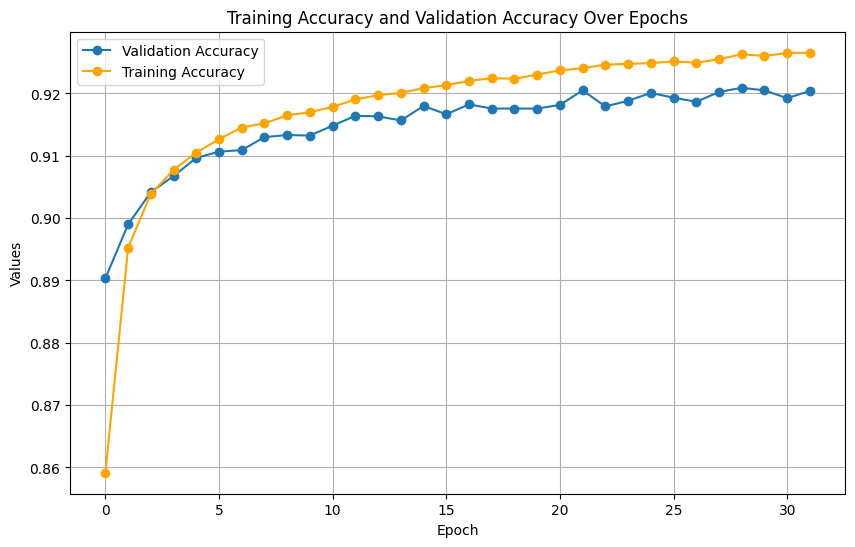
\includegraphics[width=0.8\linewidth]{include/softmax-train-val-acc.png}
  \caption{Train/Validation Accuracy for Softmax Regression}
  \label{fig:softmax_regression_acc}
\end{figure}

\begin{figure}[h]
  \centering
  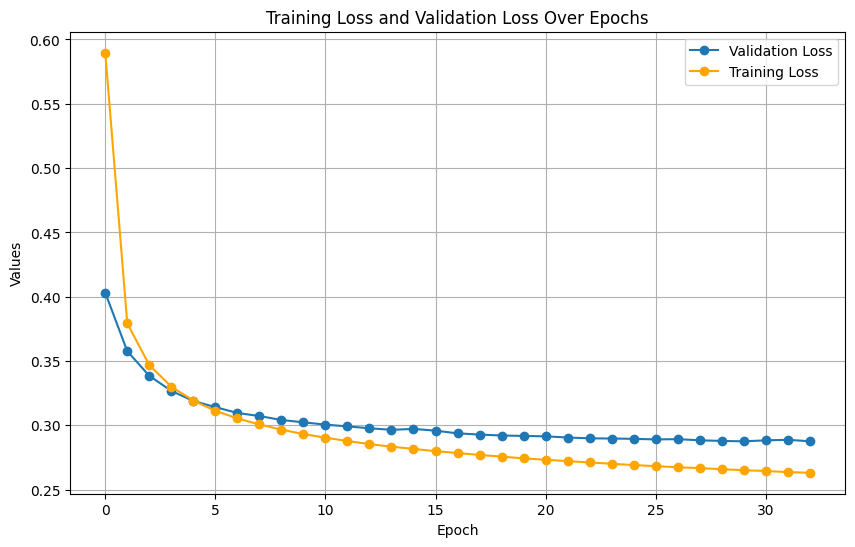
\includegraphics[width=0.8\linewidth]{include/softmax-train-val-loss.png}
  \caption{Train/Validation Loss for Softmax Regression}
  \label{fig:softmax_regression_loss}
\end{figure}

\section{Numerical Approximation of the Gradient}
To check whether our implementation of the backpropagation
is correct, we will use numerical approximation to check
the weights of the network. The numerical approximation
is done by using the following formula:
\begin{equation}
  \frac{\partial E^n}{\partial w}(w) \approx \frac{E^n(w + \epsilon) - E^n(w- \epsilon)}{2\epsilon}
\end{equation}

After perfoming the numerical approximation with $\epsilon = 1e^{-2}$, these are the 
weights for a few selected weights in the network that 
we decided to check:

% make a table
\begin{table}
  \caption{Numerical Approximation of the Gradient}
  \label{tab:approx_grad}
  \centering
  \begin{tabular}{|l|l|l|l|l|l|}
    \toprule
    Layer & Weights & Numerical Approximation & Backpropagation & Difference & Within $\epsilon^2$?\\
    \midrule
    Output & Bias & $0.099881709278$ & $0.099880510195$ & $1.19908287898e^{6}$ &  Yes\\
    \midrule
    Output & Weights 1 & $0.0097590626103$ & $0.0097590614918$ & $1.4609340039e^{-10}$ & Yes\\
    \midrule
    Output & Weights 2 & $0.004951752628$ & $0.00495175248$ & $1.4609340039e^{-10}$ & Yes\\
    \midrule
    Hidden & Bias & $0.0018200287225$ & $0.0018200877310$ & $5.900851056e^{-8}$ & Yes\\
    \midrule
    Hidden & Weights 1 & $0.0009002833399$ & $0.0009002904815$ & $7.1416564615e^{-9}$ & Yes\\
    \midrule
    Hidden & Weights 2 & $0.0009002833399$ & $0.0009002904815$ & $7.1416564615e^{-9}$ & Yes\\
    \bottomrule
  \end{tabular}
\end{table}

As we can see from \hyperref[tab:approx_grad]{Table \ref{tab:approx_grad}} the
we can see that all the backpropagation values are within 
$\epsilon^2$ of the numerical approximation. This means that our
implementation of the backpropagation is correct.

The hyperparameters for the network with mini-batch SGD are:
\begin{verbatim}
  activation = 'tanh'
  learning_rate = 1
  batch_size = 128
  epochs = 100
  early_stop = True
  early_stop_epochs = 5
  L2_penalty = 0.0
  momentum = False
  momentum_gamma = 0.9
\end{verbatim}

We also trained it on only 1 training sample.


\section{Momentum Experiments}
For the momentum experiments first we used a mini-batch SGD with the hyperparameters
given in \textbf{config\_6.yaml} which are as follows:
\begin{verbatim}
  learning_rate = 0.01
  batch_size = 128
  epochs = 100
  early_stop = True
  early_stop_epochs = 3
  regularization_type = None
  L2_penalty = 0.0
  L1_penalty = 0.0
  momentum = True
  momentum_gamma = 0.9
\end{verbatim}

This yielded a test accuracy of $96.68$ and the plots for the 
loss and accuracy, they can be seen in 
\hyperref[fig:momentum_acc]{Figure \ref{fig:momentum_acc}} and
\hyperref[fig:momentum_loss]{Figure \ref{fig:momentum_loss}}.

The training took all 100 epochs and never reached the early stopping
condition. And looking at the graphs, both the training and validation
accuracy and loss experienced similar trends, where they are constantly
getting higher for accuracy and lower for loss, showing that the 
low learning rate and high momentum allowing the model to 
search for the best solution and converge to it.

\begin{figure}[h]
  \centering
  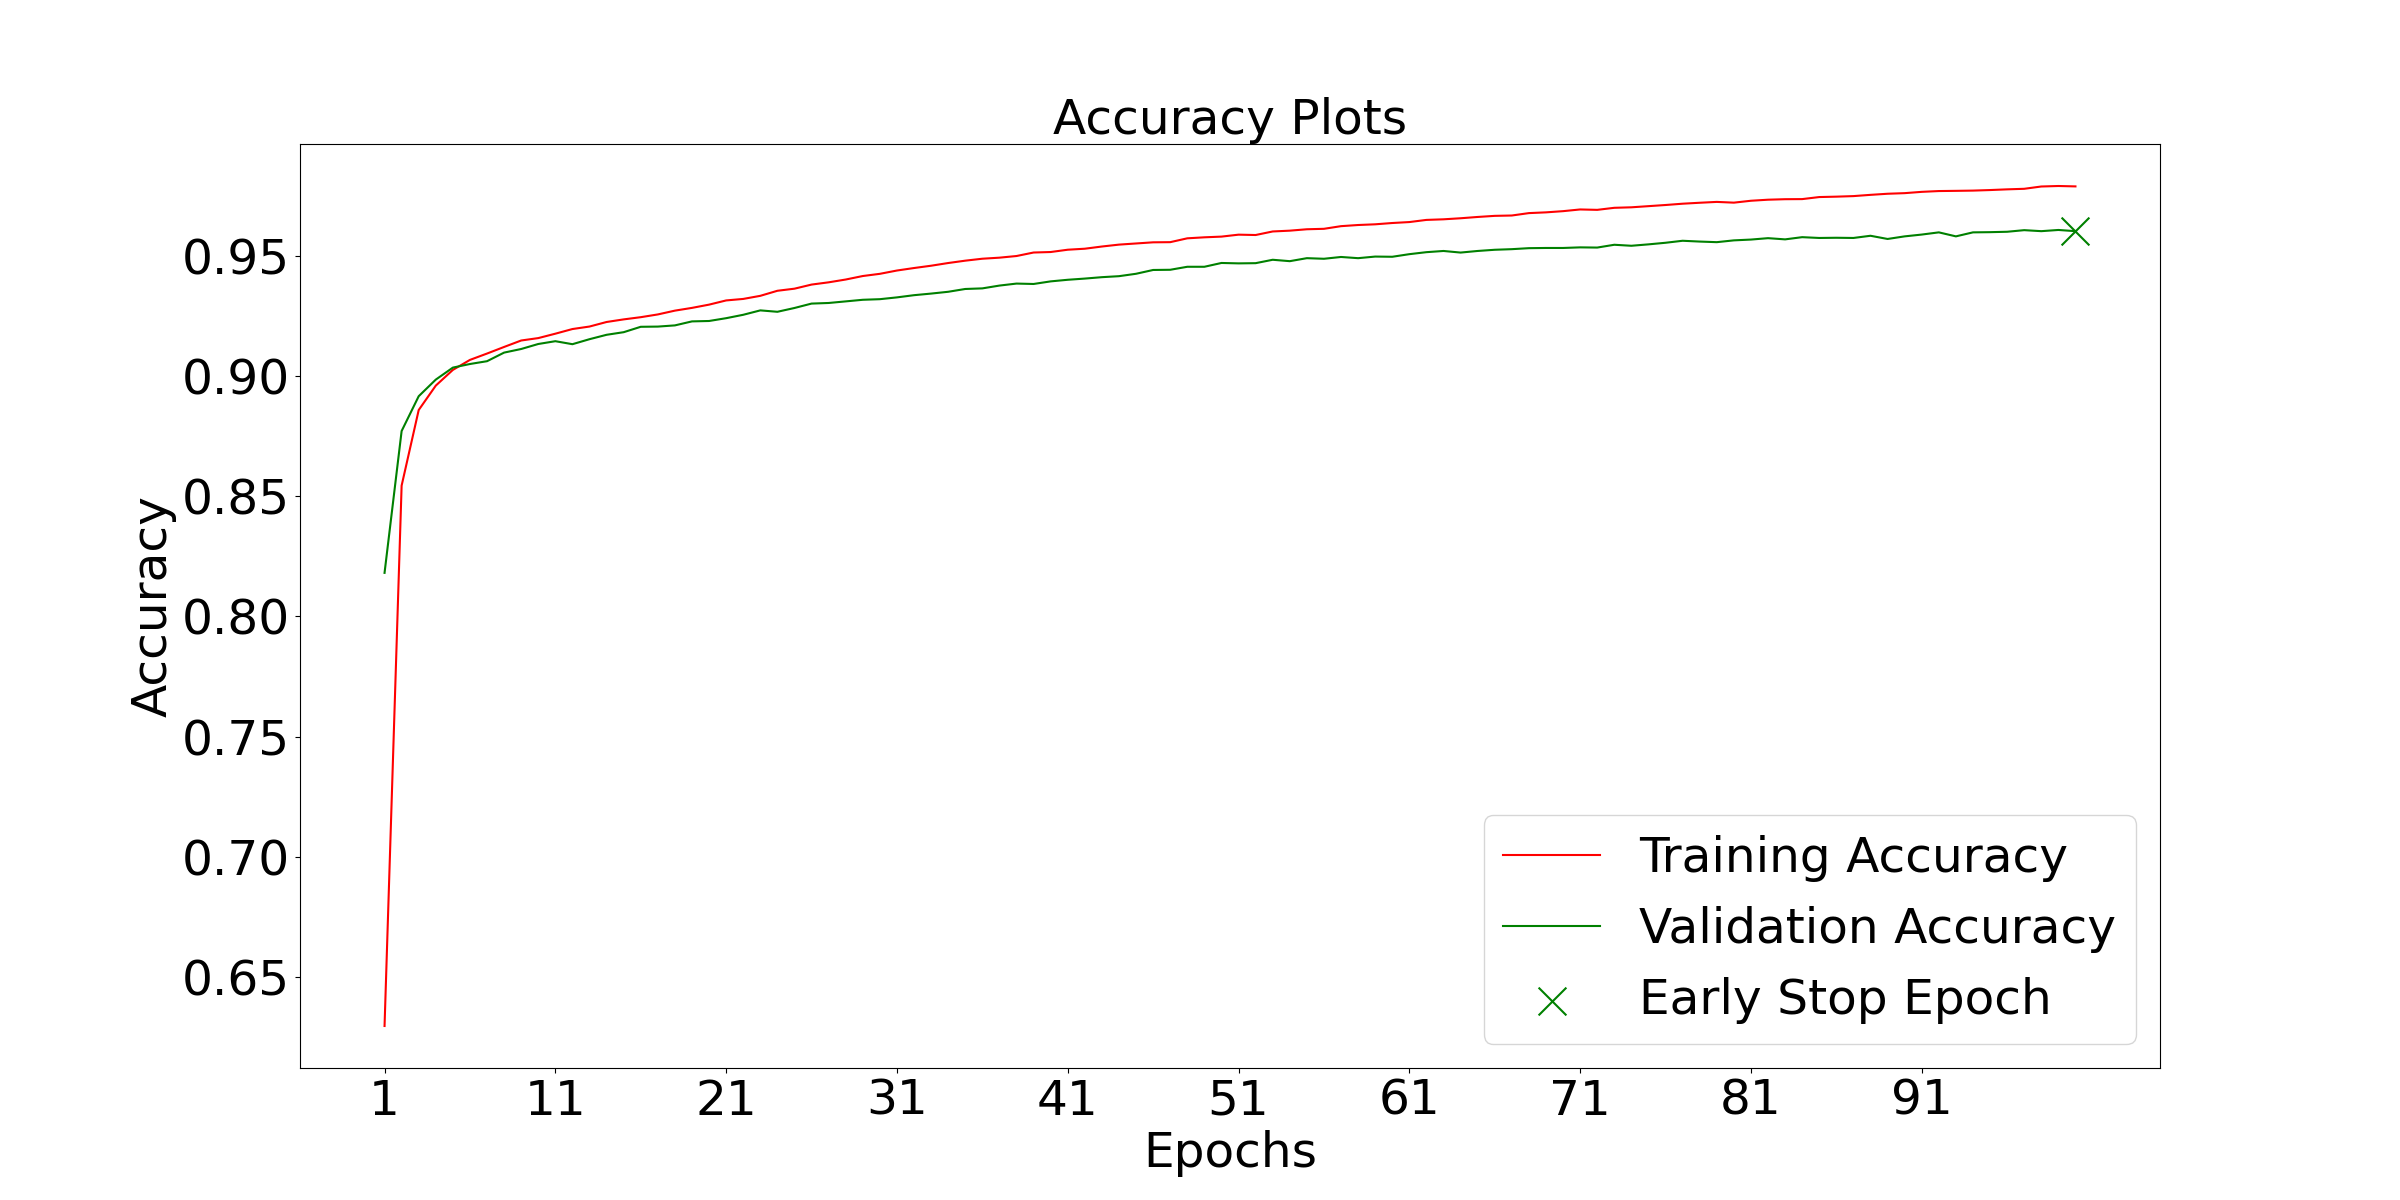
\includegraphics[width=0.8\linewidth]{include/momentum-experiments-acc.png}
  \caption{Train/Validation Accuracy for Momentum}
  \label{fig:momentum_acc}
\end{figure}


\begin{figure}[h]
  \centering
  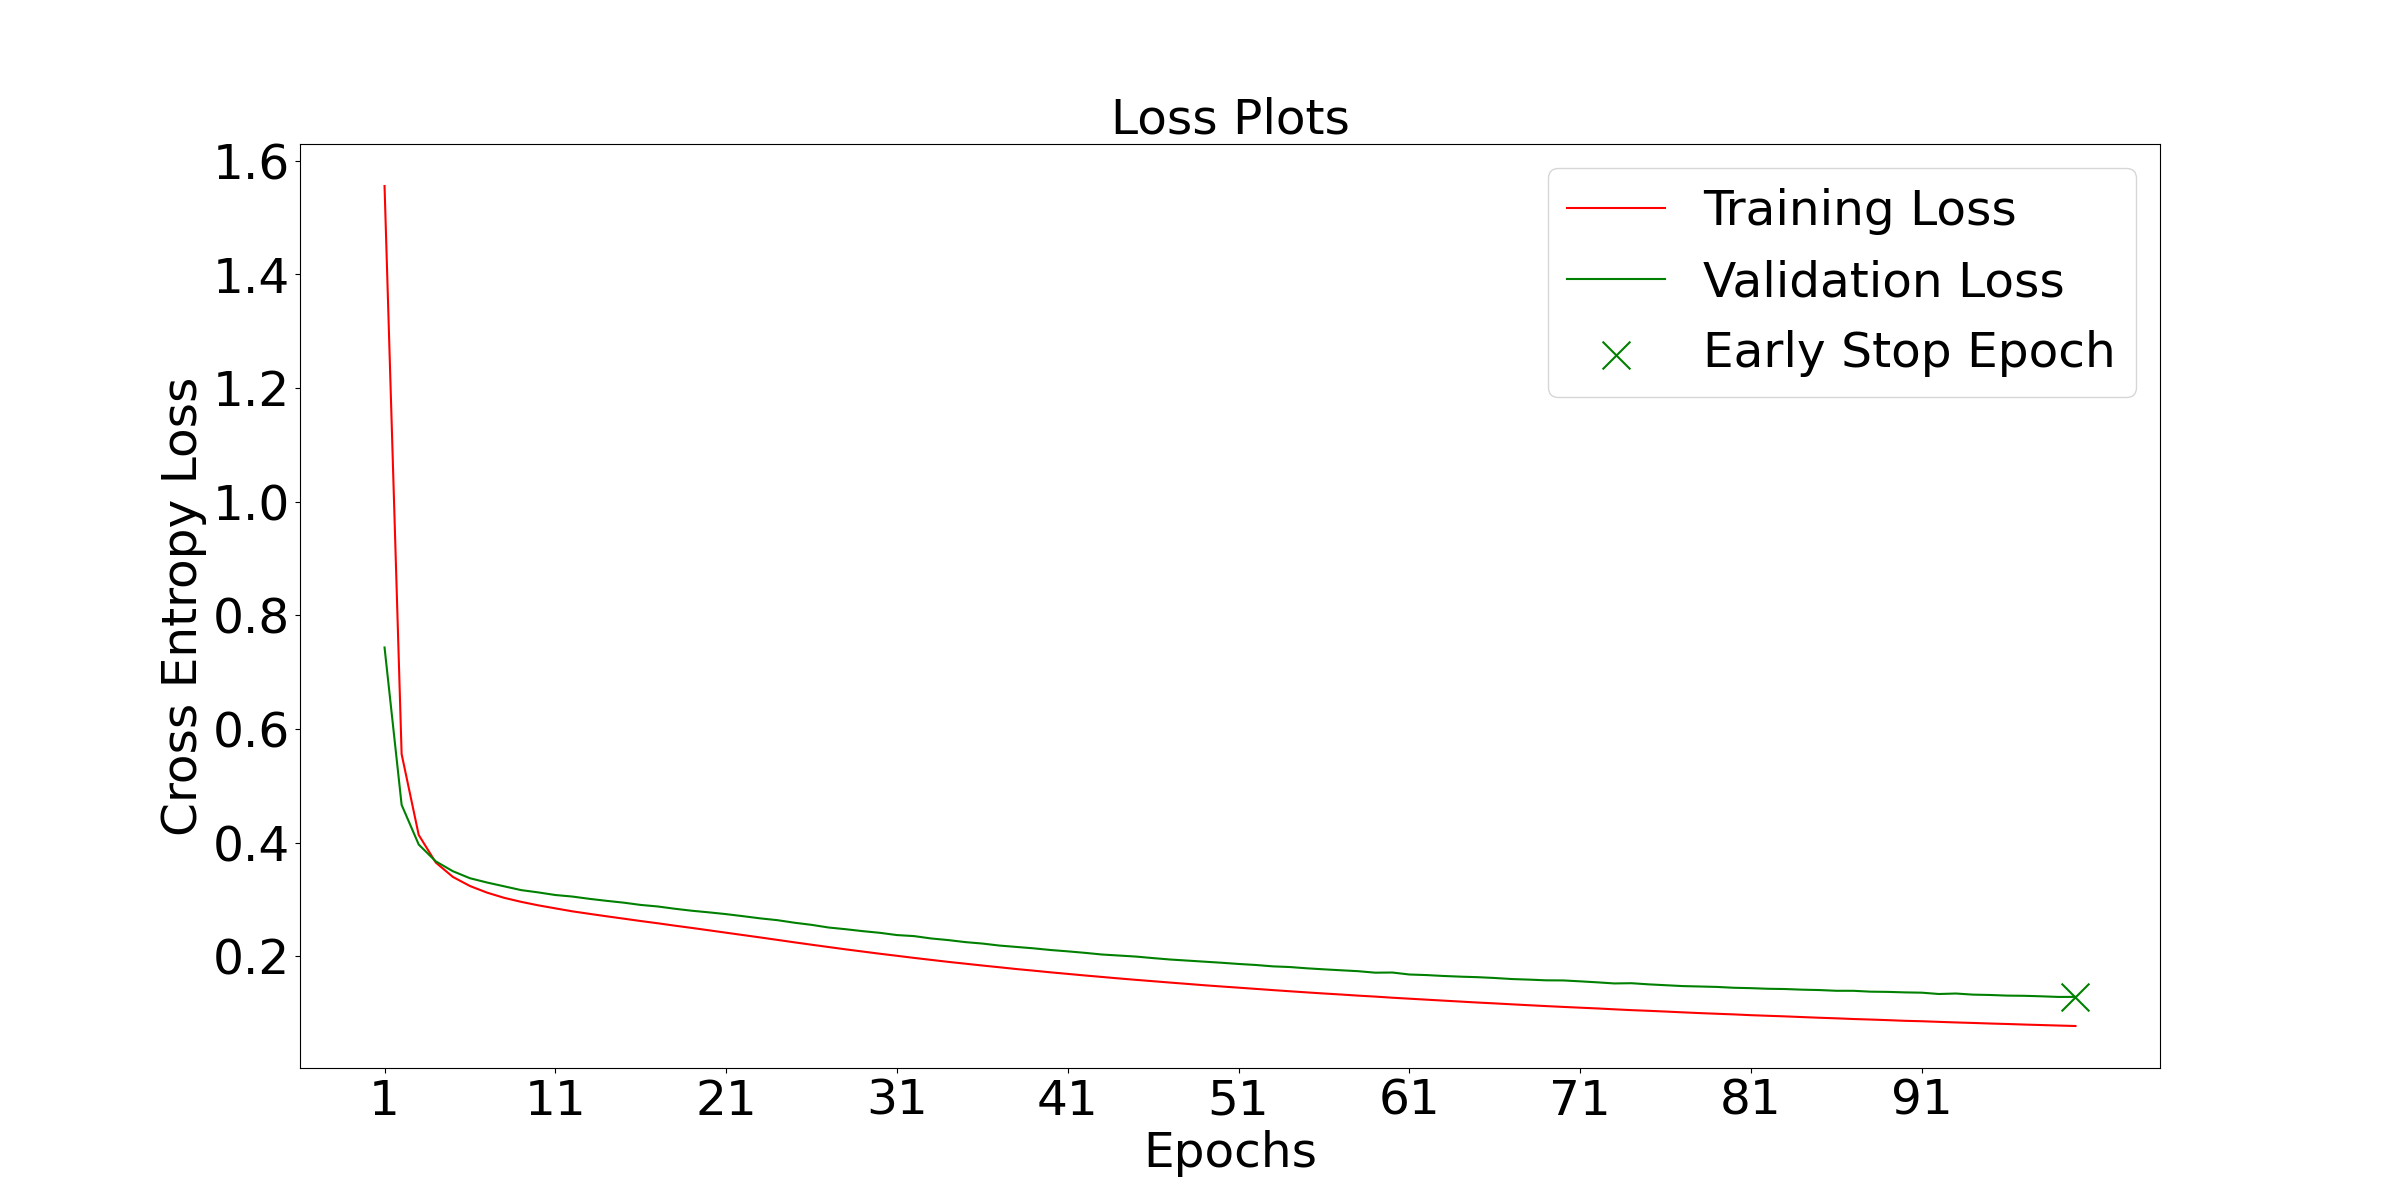
\includegraphics[width=0.8\linewidth]{include/momentum-experiments-loss.png}
  \caption{Train/Validation Loss for Momentum}
  \label{fig:momentum_loss}
\end{figure}

Then we also played around with the momentum gamma and hyperparameters
and we tried a combination where we had a small momentum gamma and a
large learning rate. The hyperparameters used are as follows:
\begin{verbatim}
  learning_rate = 0.01
  batch_size = 128
  epochs = 100
  early_stop = True
  early_stop_epochs = 3
  regularization_type = None
  L2_penalty = 0.0
  L1_penalty = 0.0
  momentum = True
  momentum_gamma = 0.01
\end{verbatim}

This yielded a test accuracy of $91.87$ instead of the $96.68$ from the previous test. This is due to the low momentum gamma that was set for the second test, this is because, with lower
momentum gamma, it makes the network more sensitive and will usually prevent the chance of overshooting the minimum. However, 
it will also lead to slower convergence which is why we see a lower test accuracy as compared to the first test.

Overall, the second test gave us a more stable and reliable model, as compared to the first test, which is why we would prefer the second test over the first test if our only goal is 
to achieve a higher test accuracy and the best possible 
model. But the tradeoff will be it's slower convergence rate.

The training plots for this can be seen in 
\hyperref[fig:momentum_acc_2]{Figure \ref{fig:momentum_acc_2}} and
\hyperref[fig:momentum_loss_2]{Figure \ref{fig:momentum_loss_2}}.

\begin{figure}[h]
  \centering
  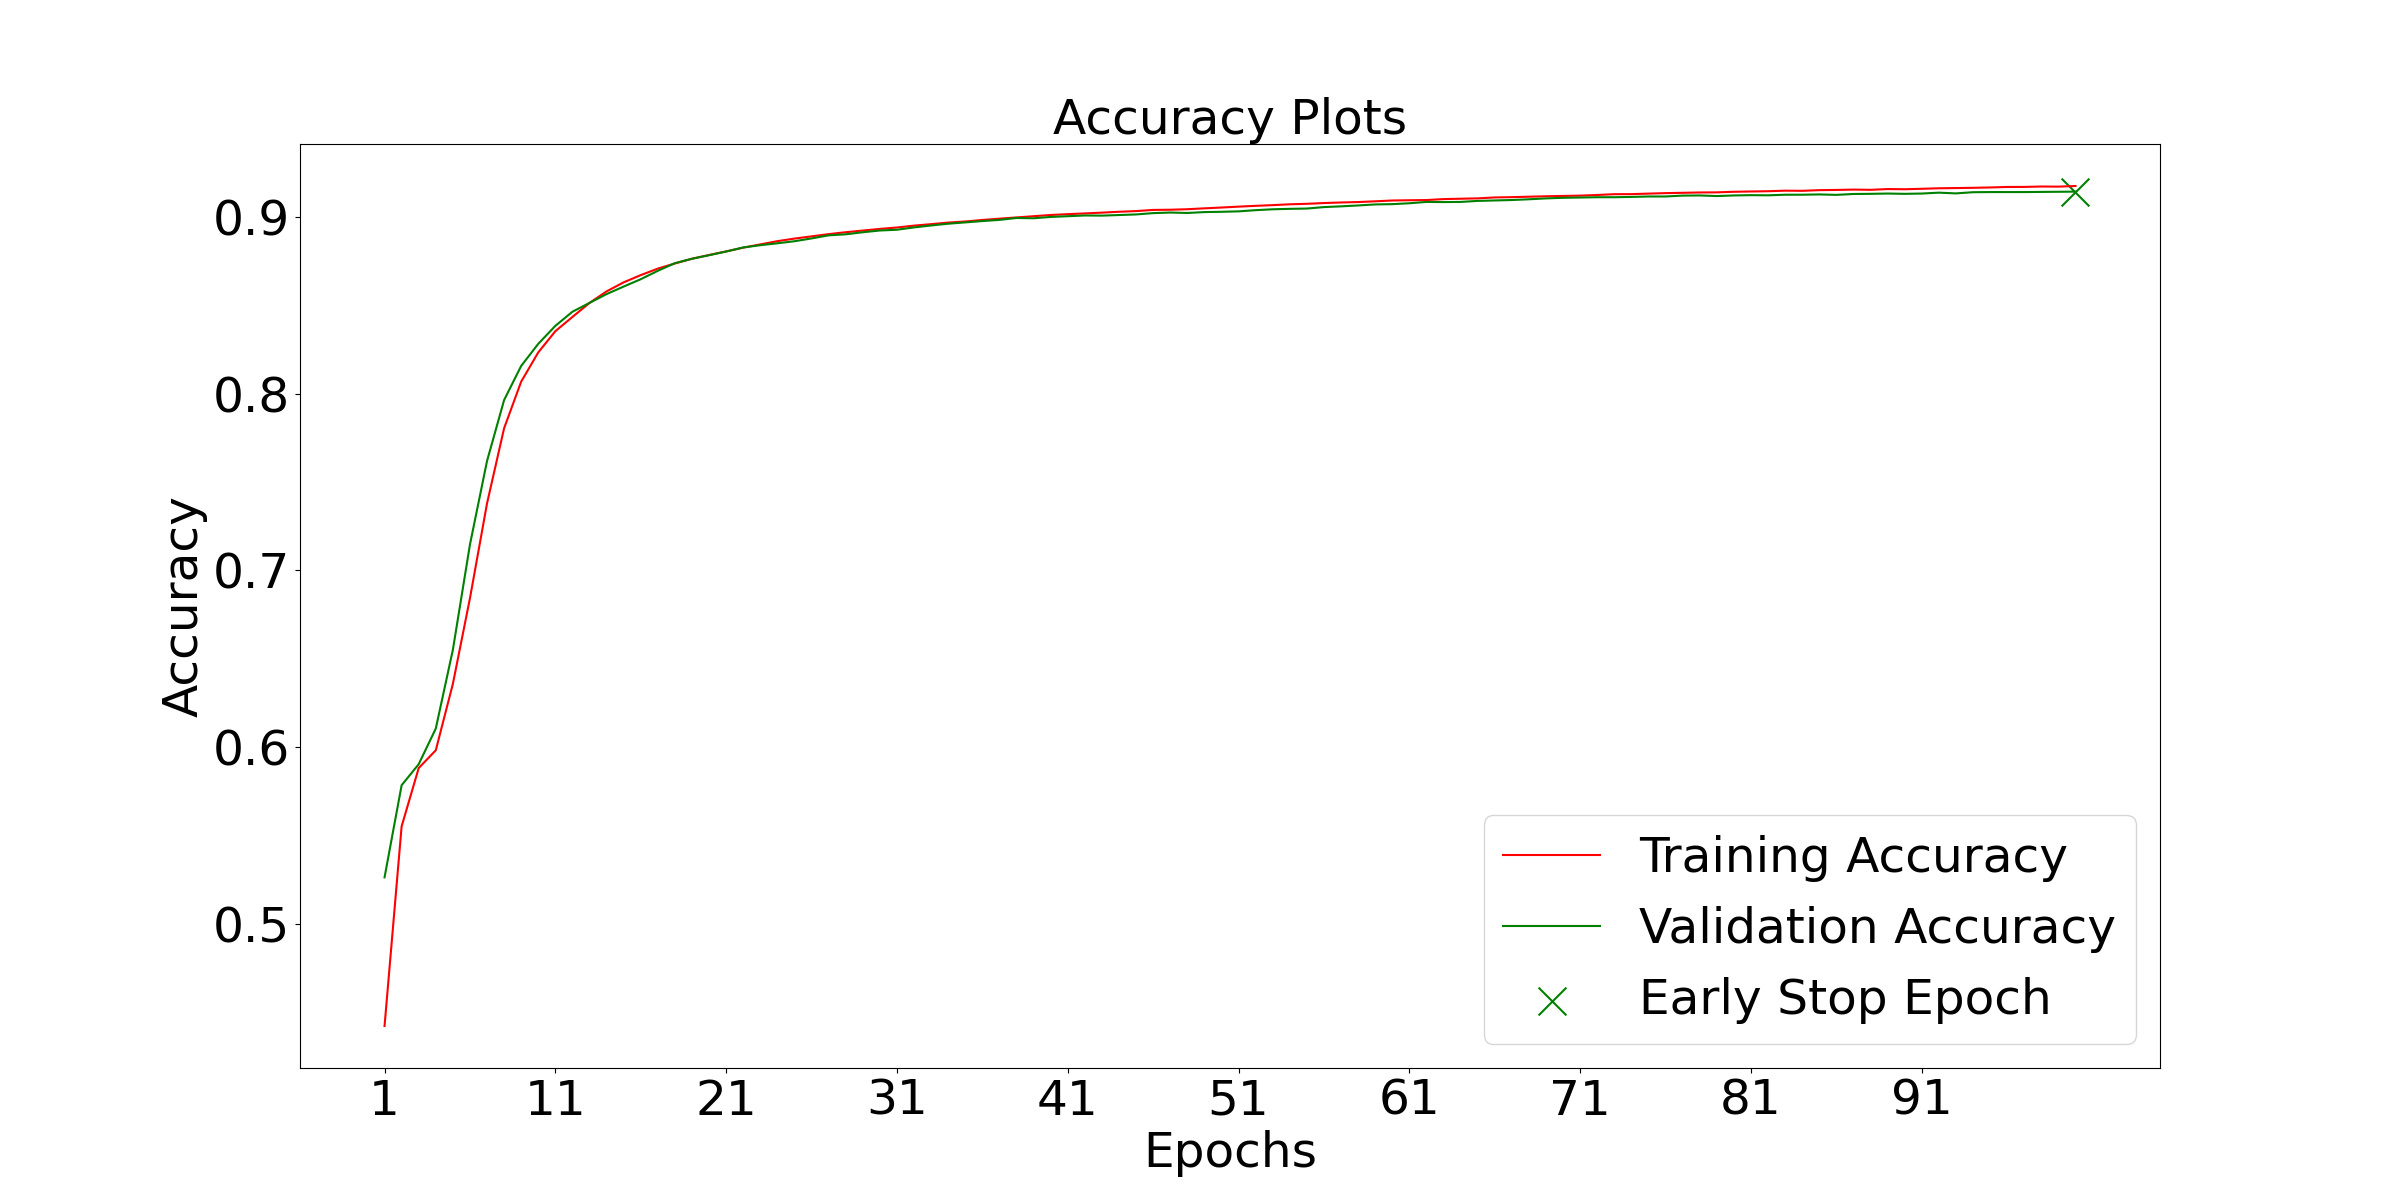
\includegraphics[width=0.8\linewidth]{include/momentum-experiments-acc-2.png}
  \caption{Train/Validation Accuracy for Momentum}
  \label{fig:momentum_acc_2}
\end{figure}

\begin{figure}[h]
  \centering
  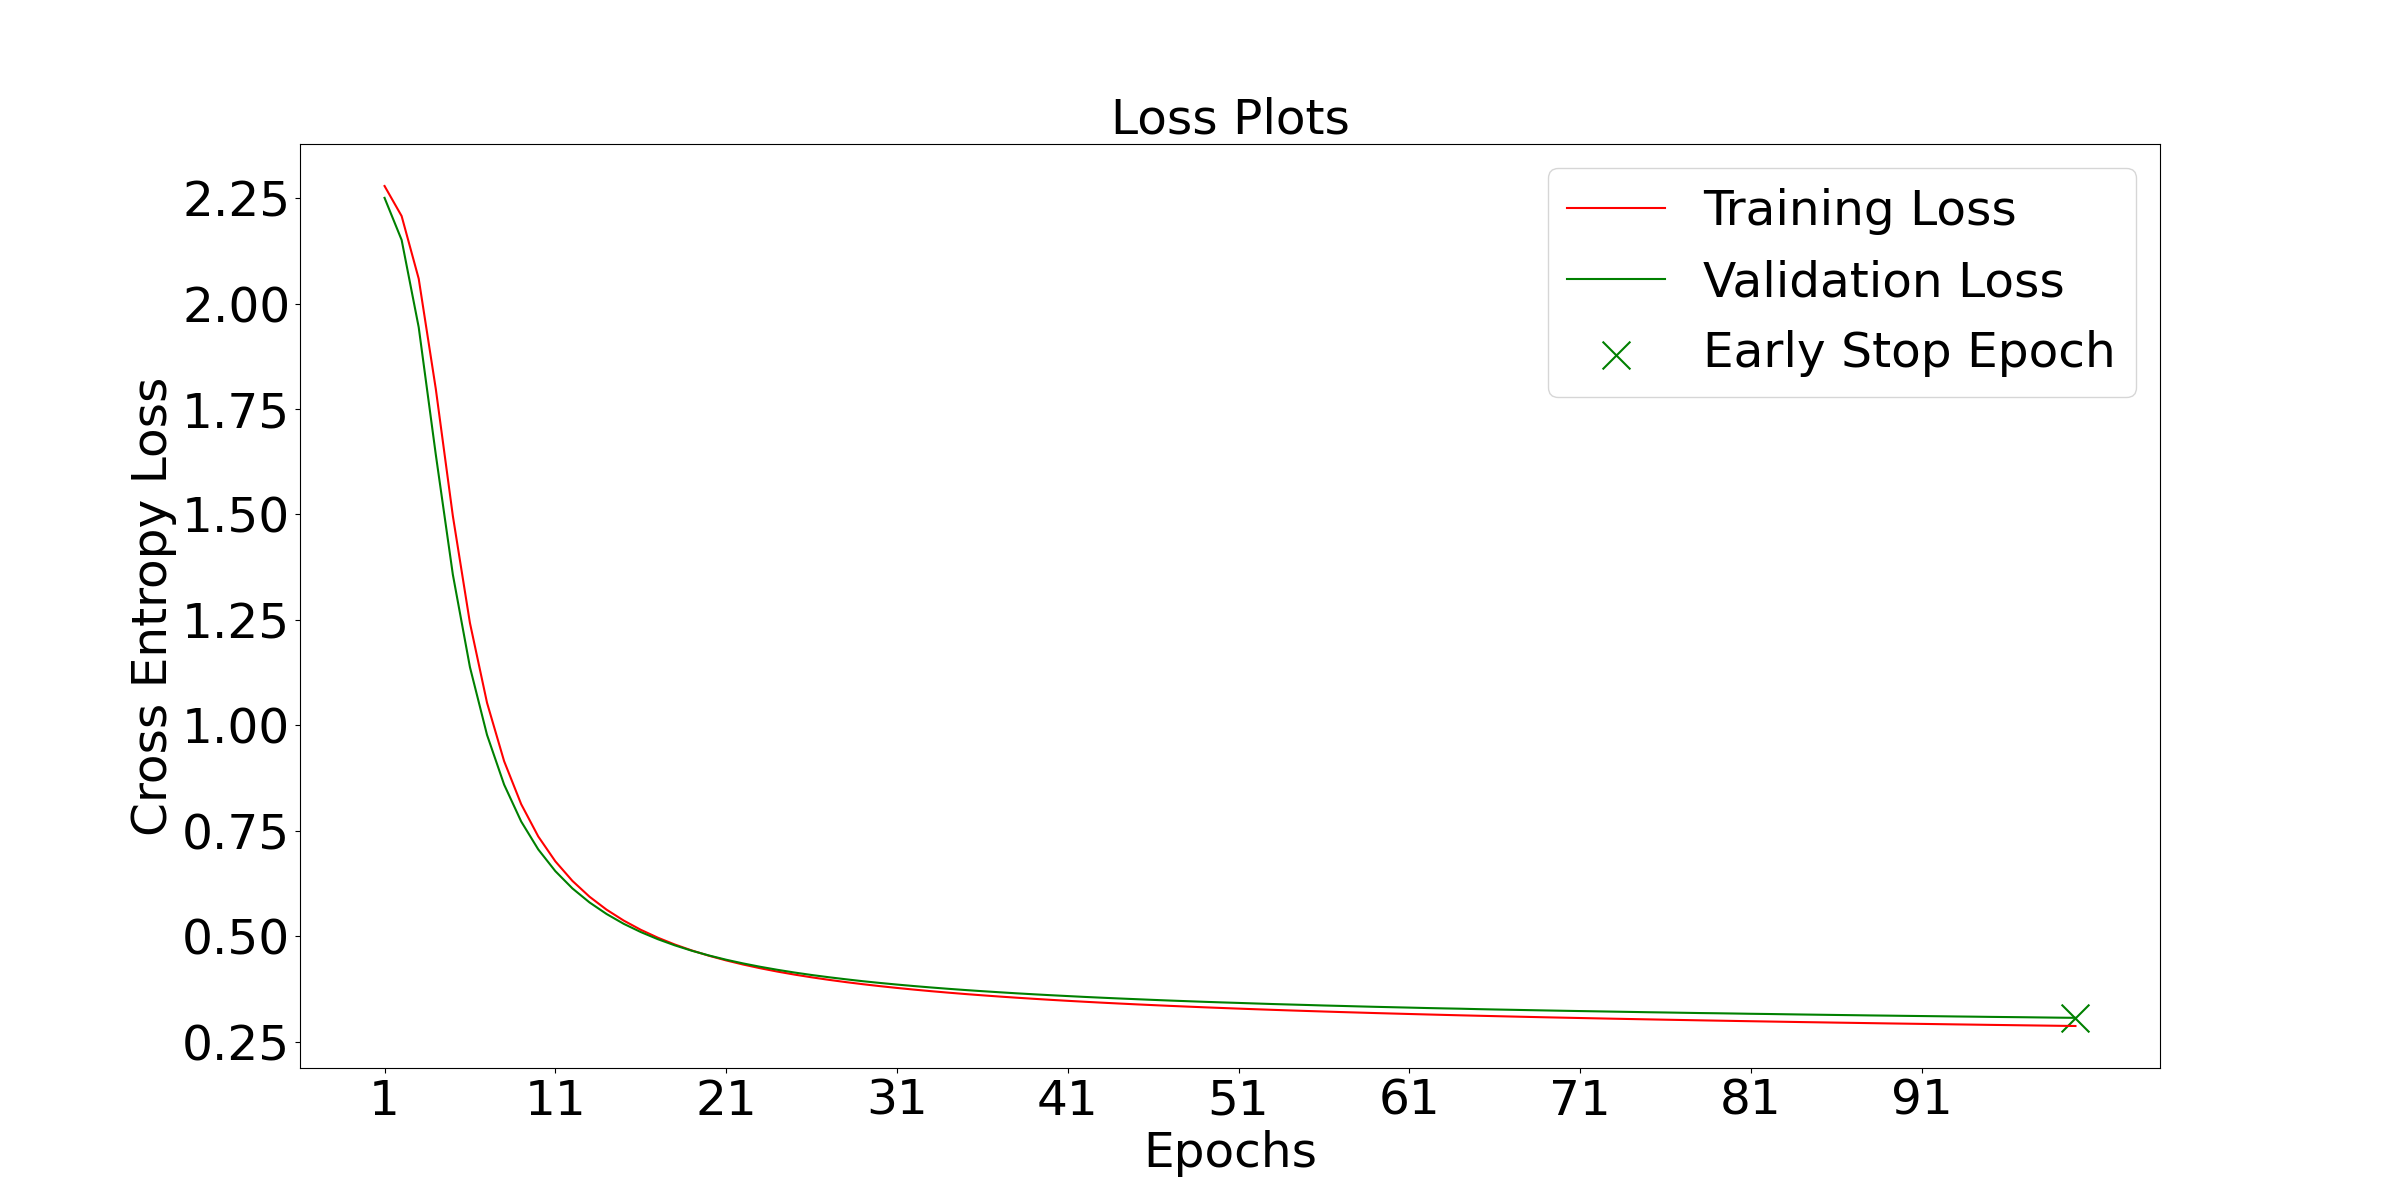
\includegraphics[width=0.8\linewidth]{include/momentum-experiments-loss-2.png}
  \caption{Train/Validation Loss for Momentum}
  \label{fig:momentum_loss_2}
\end{figure}



\section{Regularization Experiments}
In this section we did experiments with different regularization methods which are 
L2 regularization and L1 regularization. 

\subsection{L2 Regularization}
For L2 regularization we SGD with mini-batches and used the following hyperparameters:
\begin{verbatim}
  learning_rate = 0.01
  batch_size = 128
  epochs = 110
  early_stop = True
  early_stop_epochs = 3
  regularization_type = 'L2'
  L2_penalty = 0.01
  L1_penalty = 0.01
  momentum = True
  momentum_gamma = 0.9
\end{verbatim}

This yielded a test accuracy of $0.9699$ and a test loss of 
$0.10277824069050659$ the plots for the the loss and accuracy can be seen in
\hyperref[fig:l2_acc]{Figure \ref{fig:l2_acc}} and
\hyperref[fig:l2_loss]{Figure \ref{fig:l2_loss}}.

\begin{figure}[h]
  \centering
  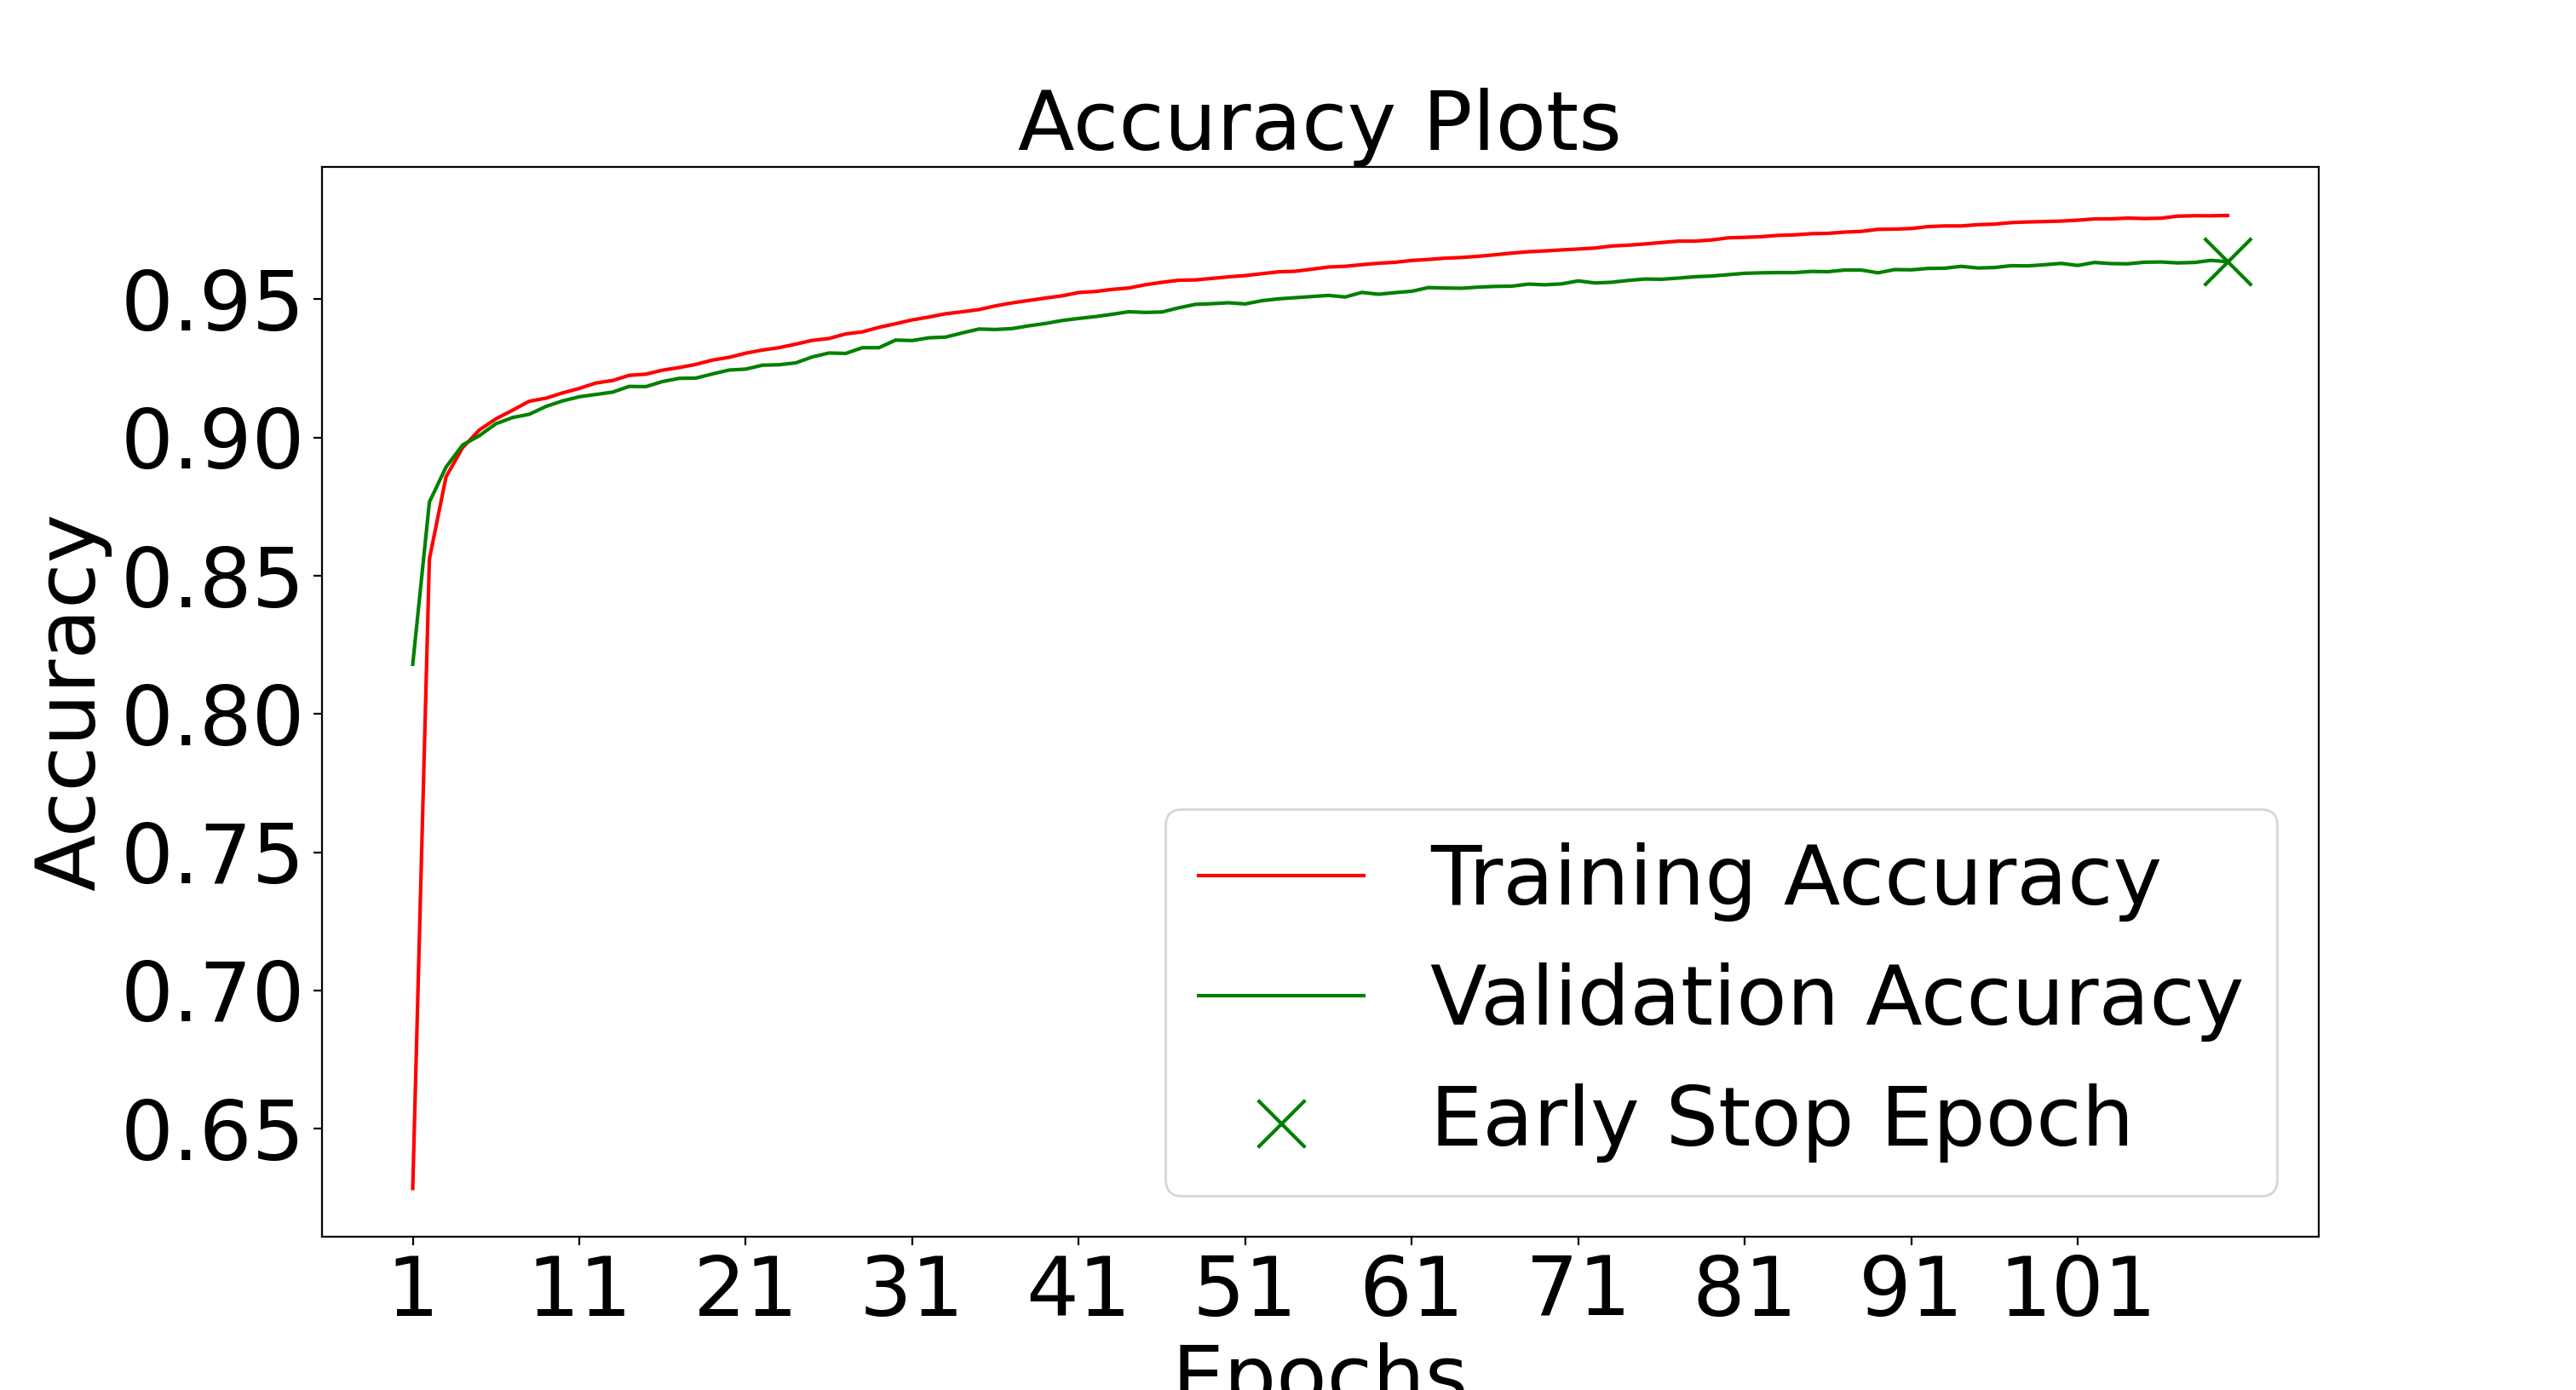
\includegraphics[width=0.8\linewidth]{include/reg-exp-l2-acc.png}
  \caption{Train/Validation Accuracy for L2 Regularization}
  \label{fig:l2_acc}
\end{figure}

\begin{figure}[h]
  \centering
  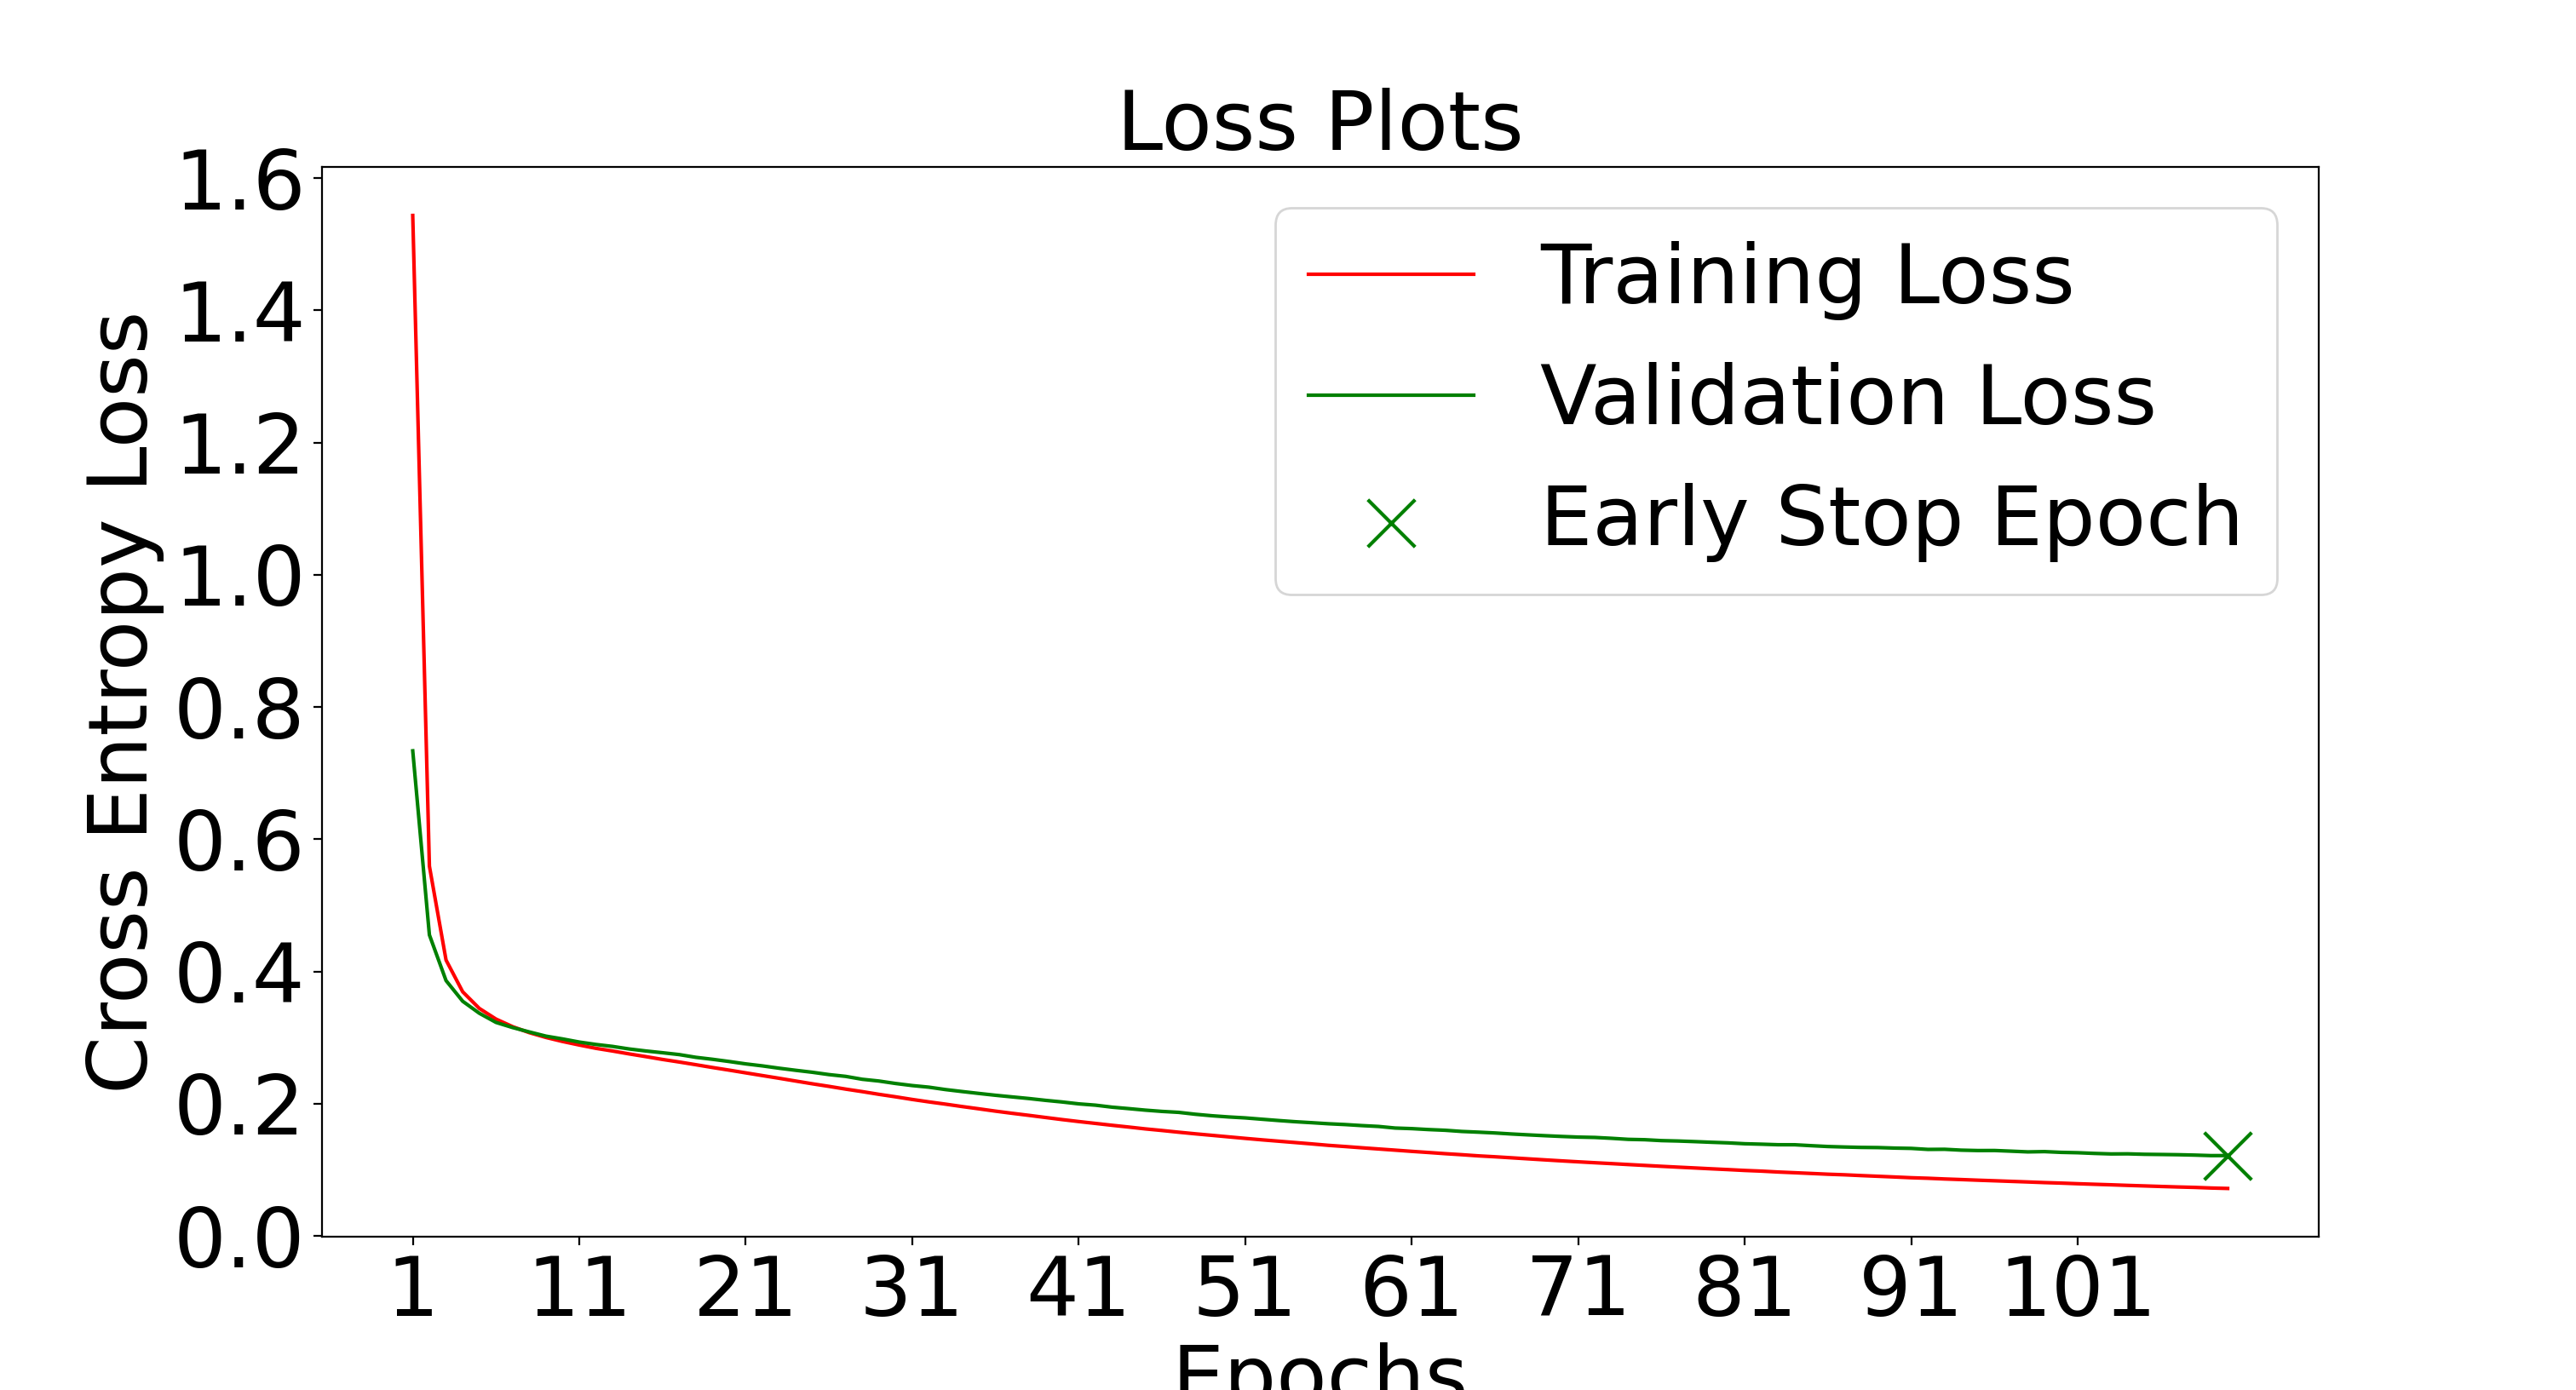
\includegraphics[width=0.8\linewidth]{include/reg-exp-l2-loss.png}
  \caption{Train/Validation Loss for L2 Regularization}
  \label{fig:l2_loss}
\end{figure}


\subsection{L1 Regularization}
For L1 regularization we used the same hyperparameters as L2 regularization
except we changed the regularization type to L1 and increased 
epochs from $110$ to $160$ to see if how much more decay L1 adds versus
L2. This yielded a test accuracy of
$0.9737$ and a test loss of $0.08931316605518423$ the plots for the loss and accuracy
can be seen in \hyperref[fig:l1_acc]{Figure \ref{fig:l1_acc}} and
\hyperref[fig:l1_loss]{Figure \ref{fig:l1_loss}}.

\begin{figure}[h]
  \centering
  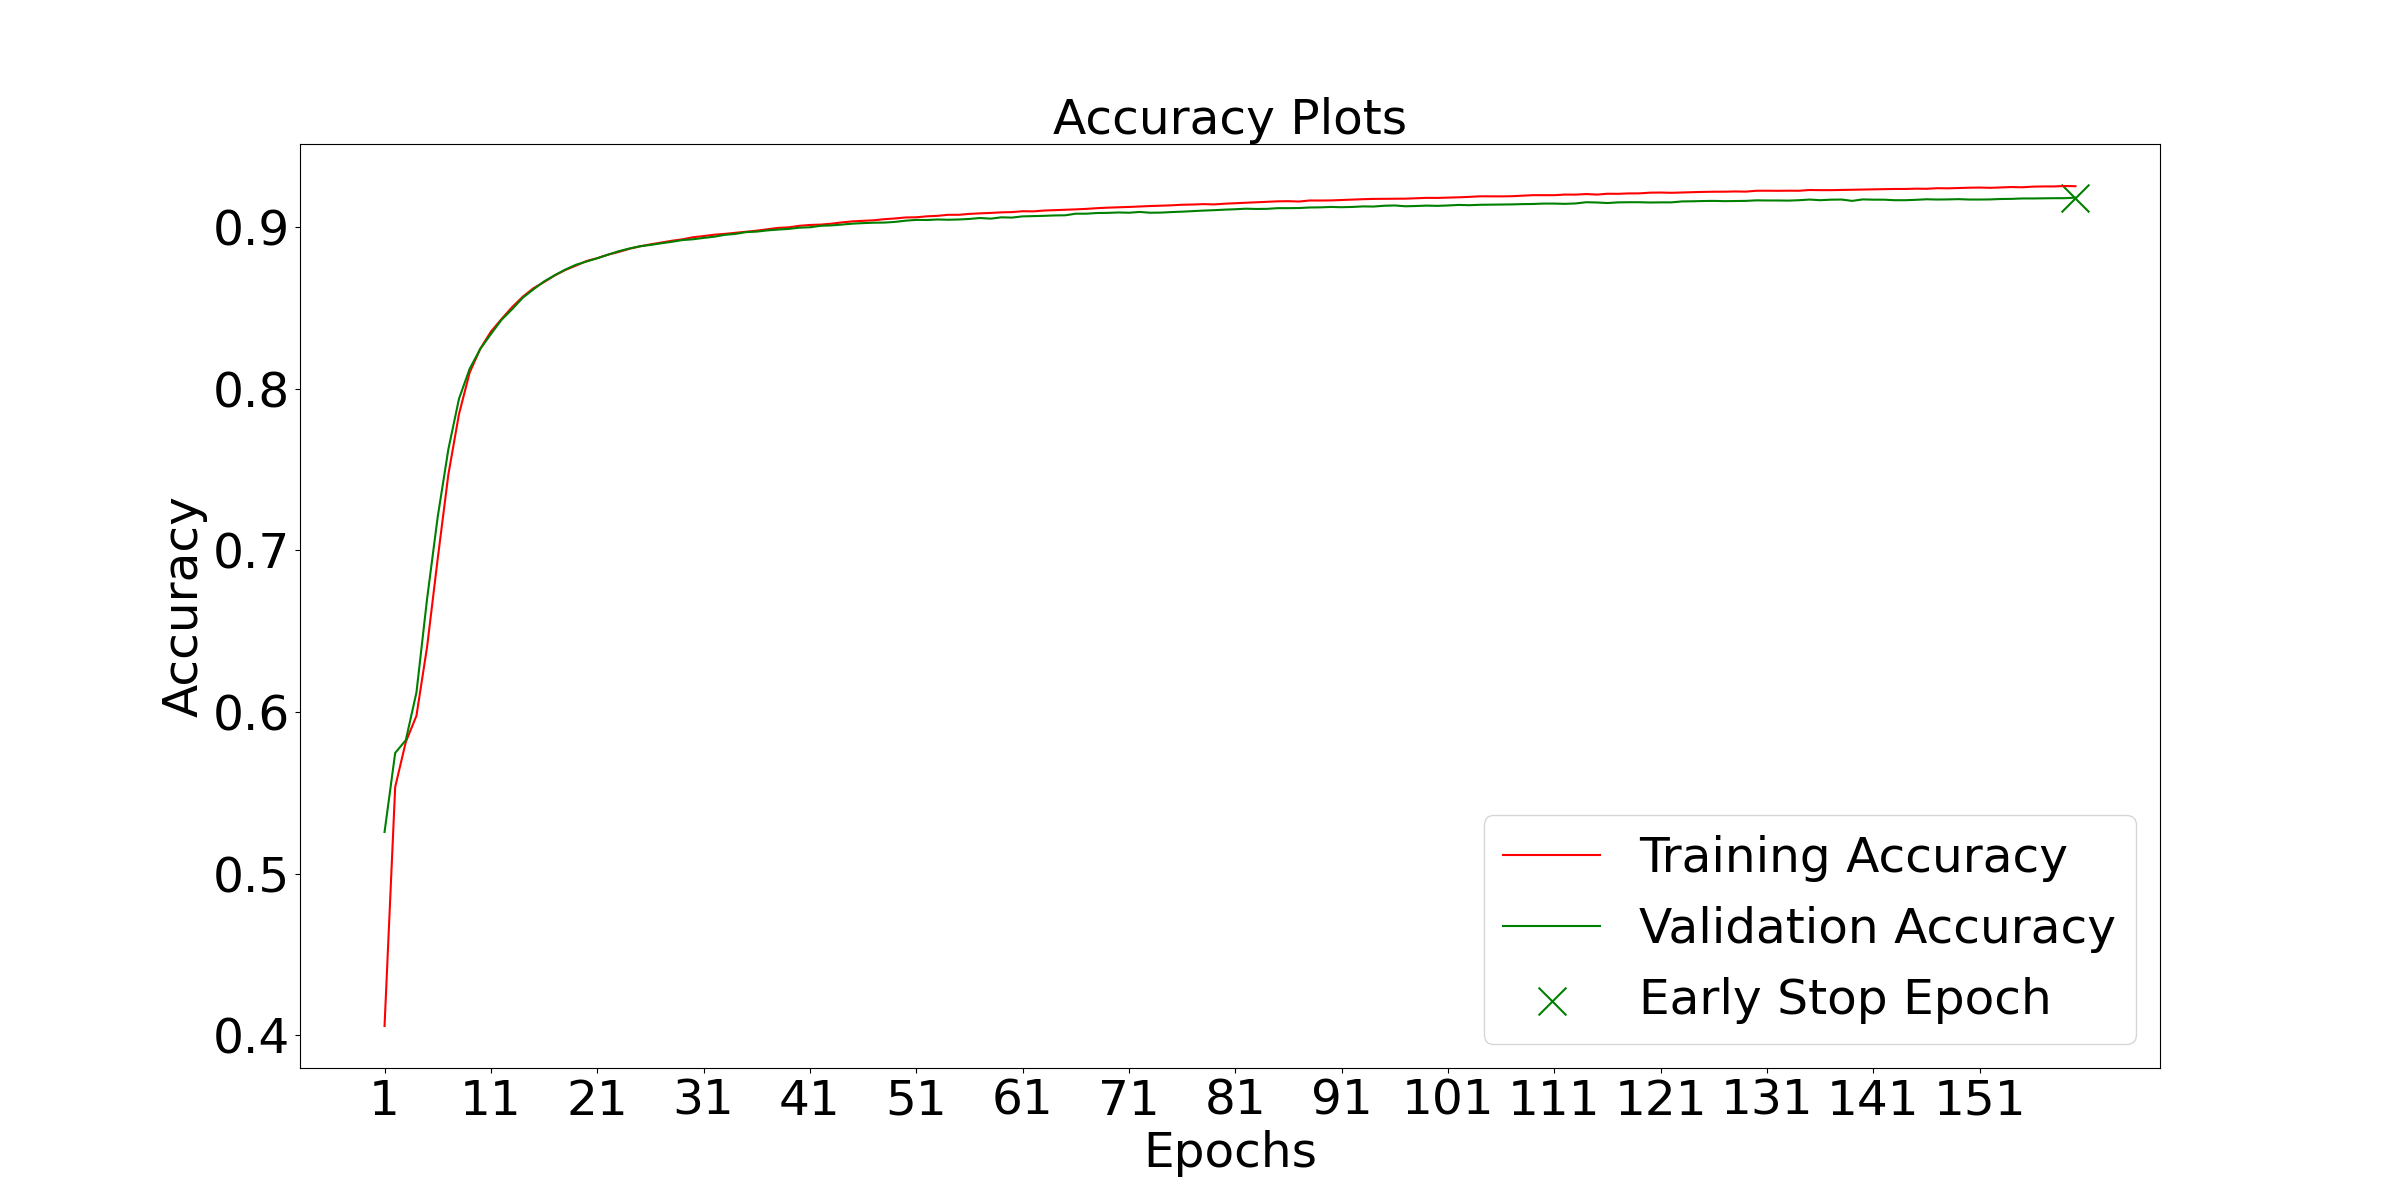
\includegraphics[width=0.8\linewidth]{include/reg-exp-l1-acc.png}
  \caption{Train/Validation Accuracy for L1 Regularization}
  \label{fig:l1_acc}
\end{figure}

\begin{figure}[h]
  \centering
  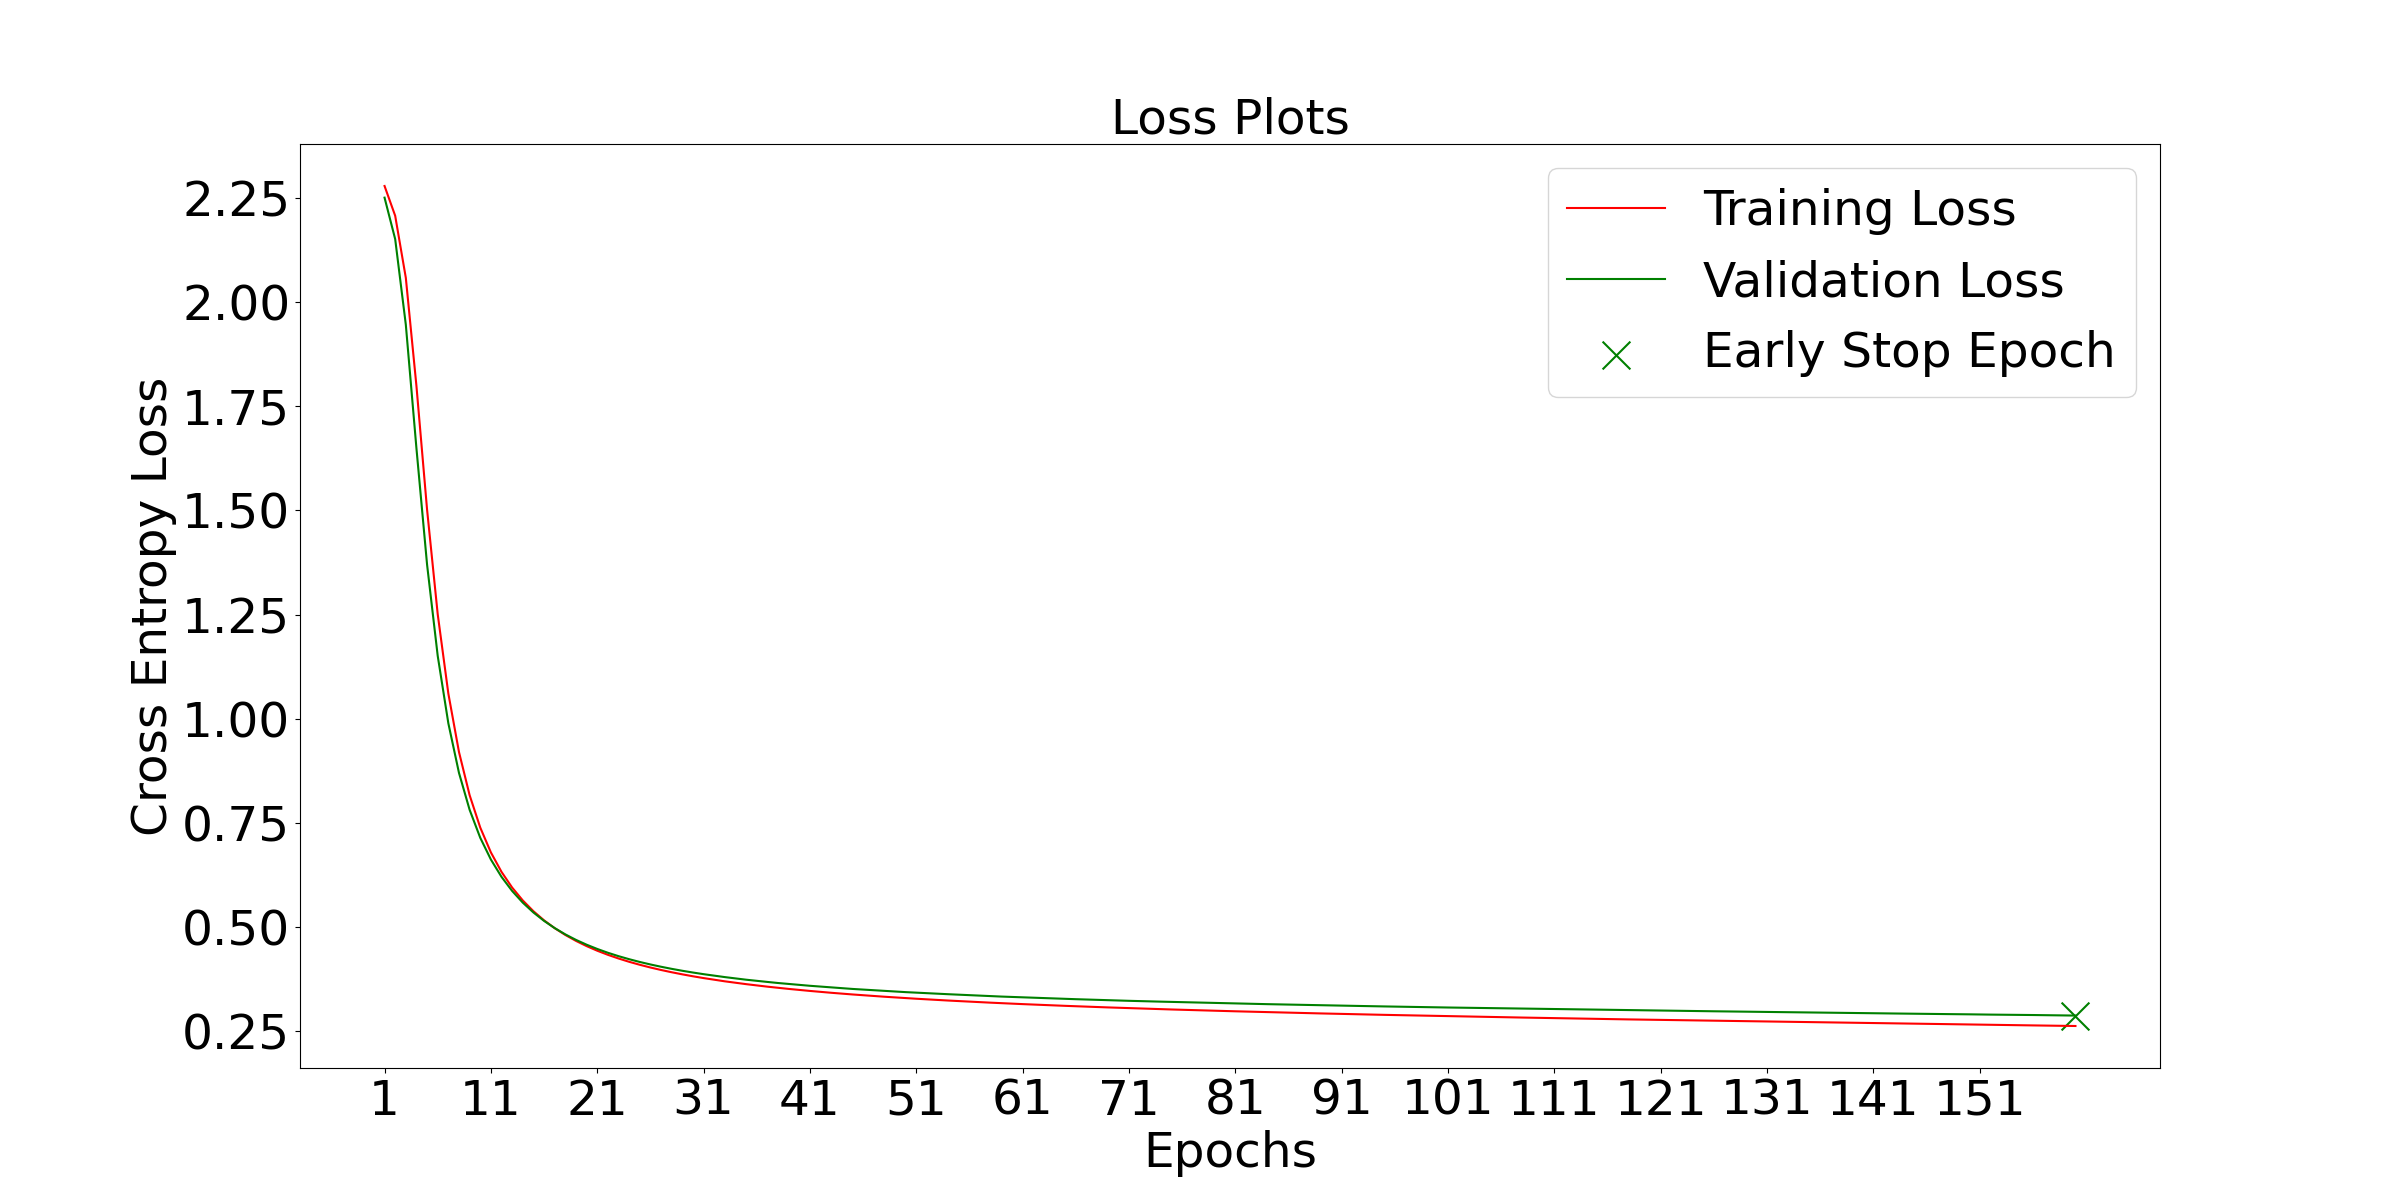
\includegraphics[width=0.8\linewidth]{include/reg-exp-l1-loss.png}
  \caption{Train/Validation Loss for L1 Regularization}
  \label{fig:l1_loss}
\end{figure}

\subsection{L2 with smaller $\lambda$}
For this experiment we used the same hyperparameters as the L2 regularization
experiment except we changed the L2 penalty from $0.01$ to $0.0001$. This yielded
a test accuracy of $0.9713$ and a test loss of $0.10168974708457909$, 
the plots for this can be seen in \hyperref[fig:l2_2_acc]{Figure \ref{fig:l2_2_acc}} and
\hyperref[fig:l2_2_loss]{Figure \ref{fig:l2_2_loss}}.

\begin{figure}[h!]
  \centering
  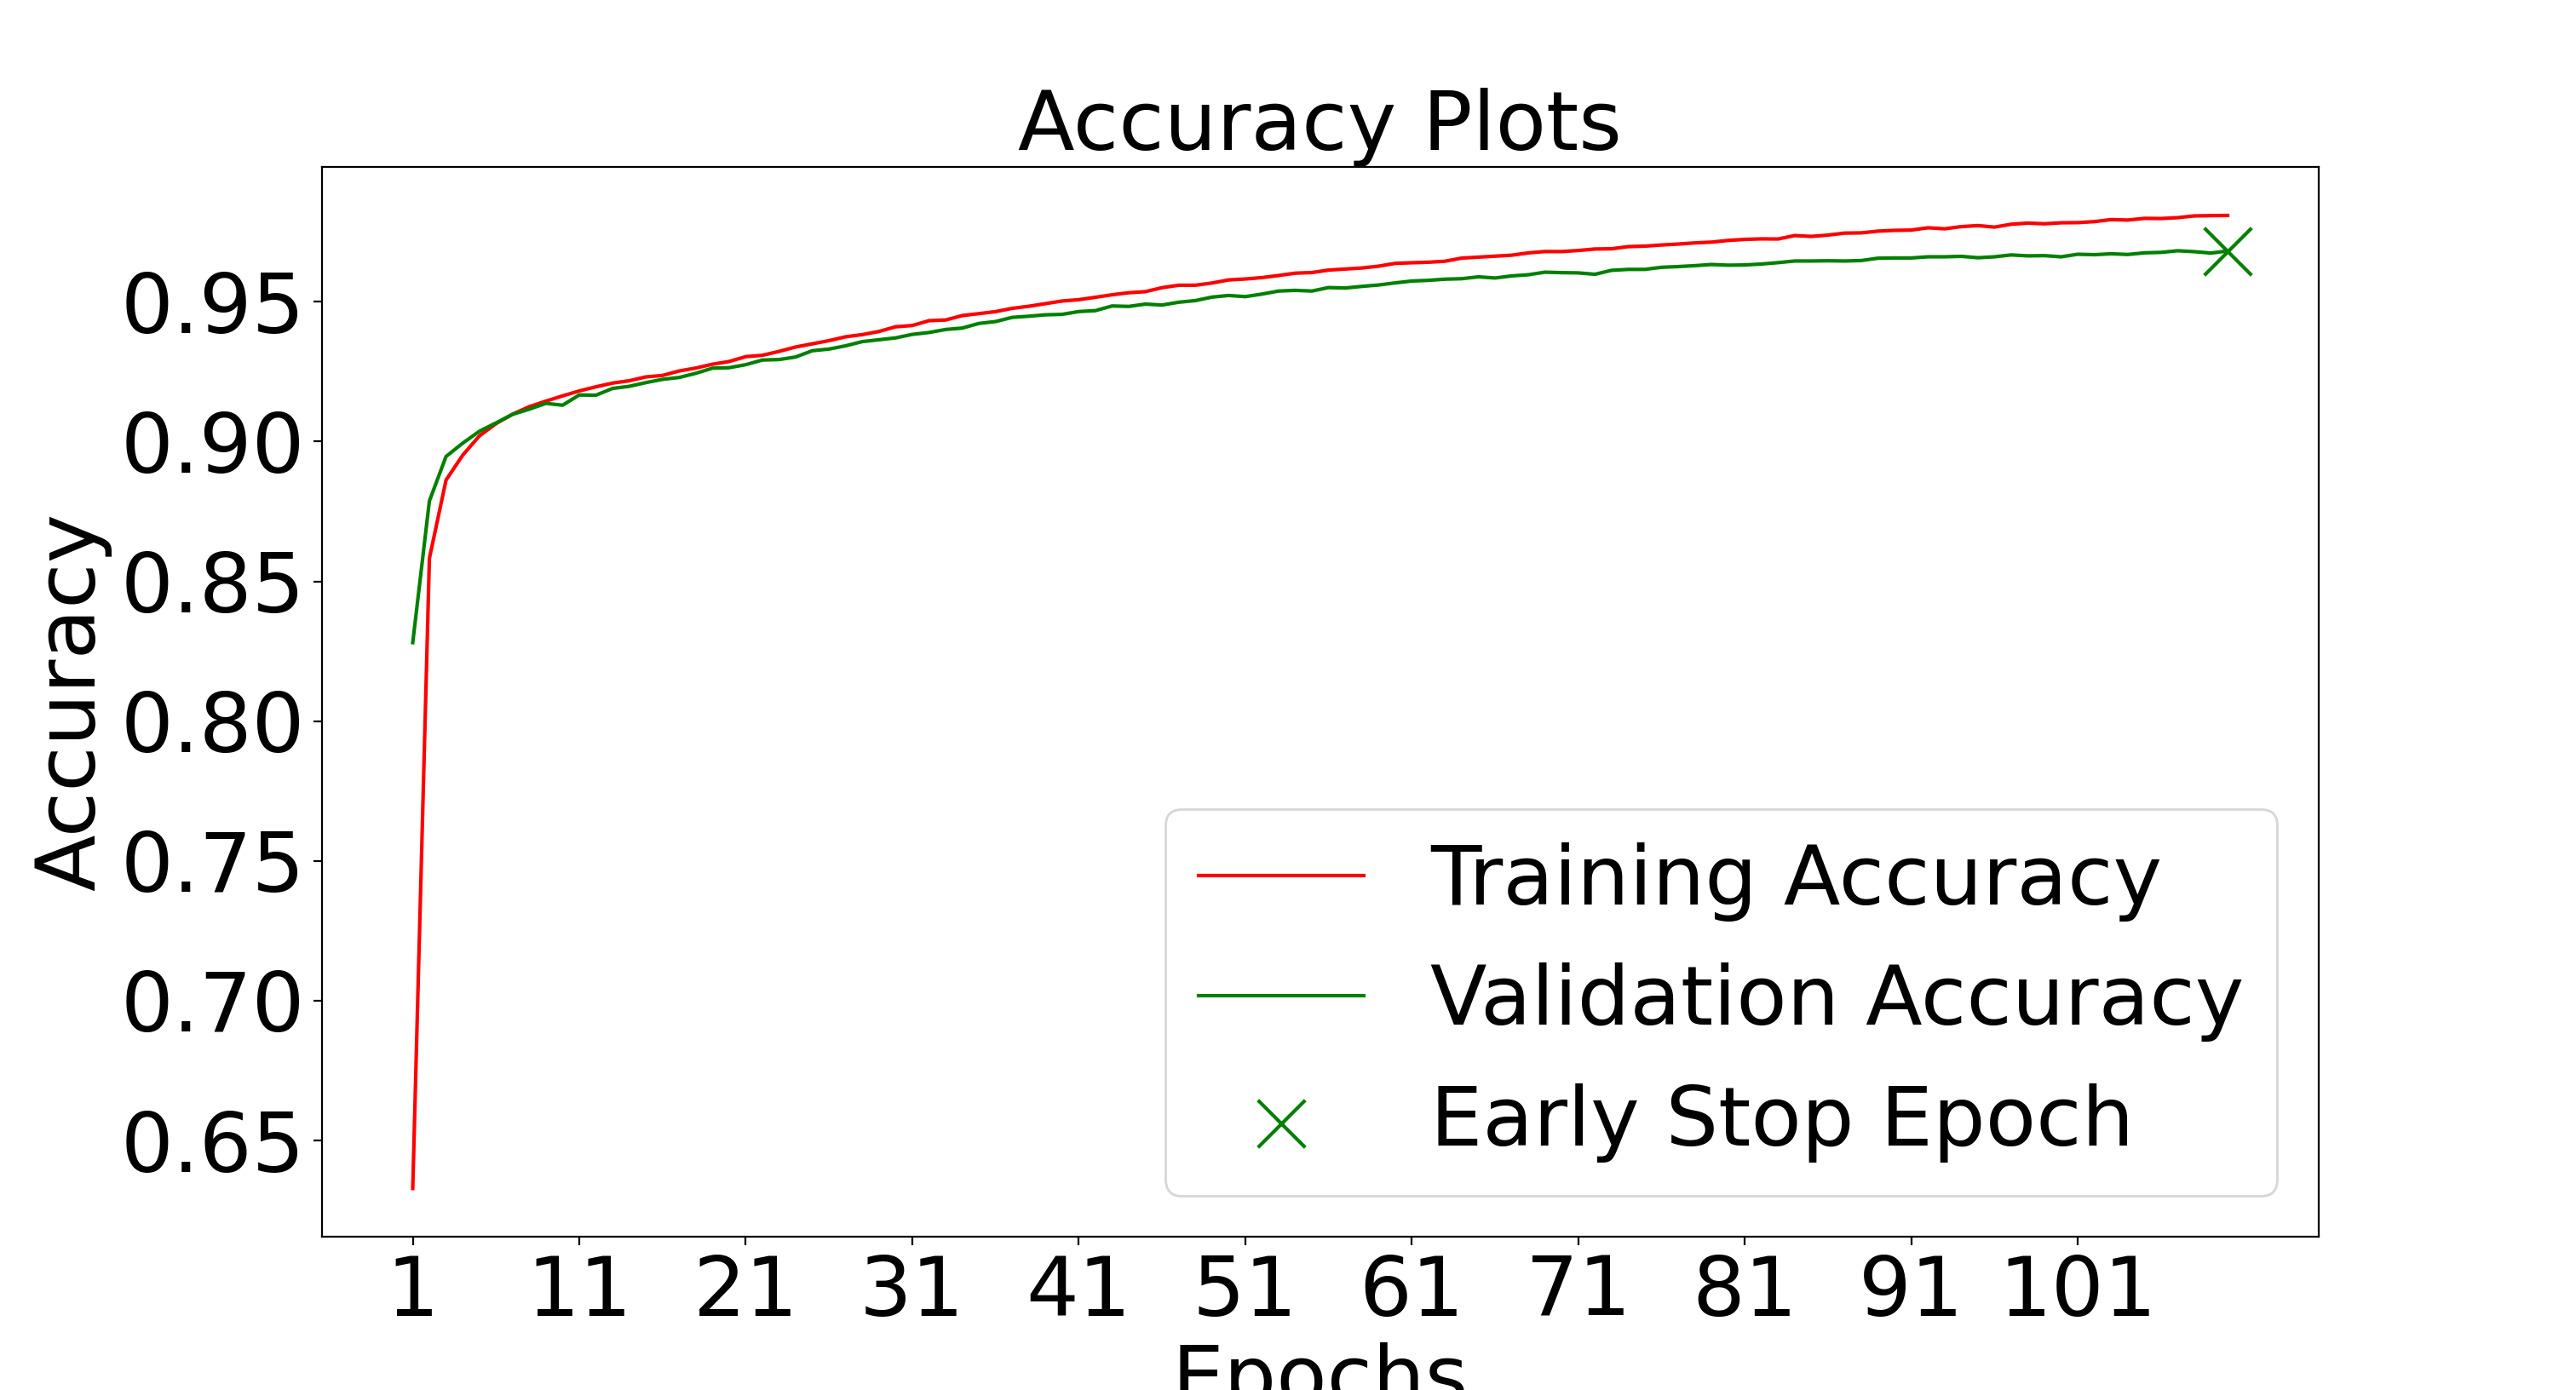
\includegraphics[width=0.8\linewidth]{include/reg-exp-l2-2-acc.png}
  \caption{Train/Validation Accuracy for L2 Regularization with smaller $\lambda$}
  \label{fig:l2_2_acc}
\end{figure}

\begin{figure}[h!]
  \centering
  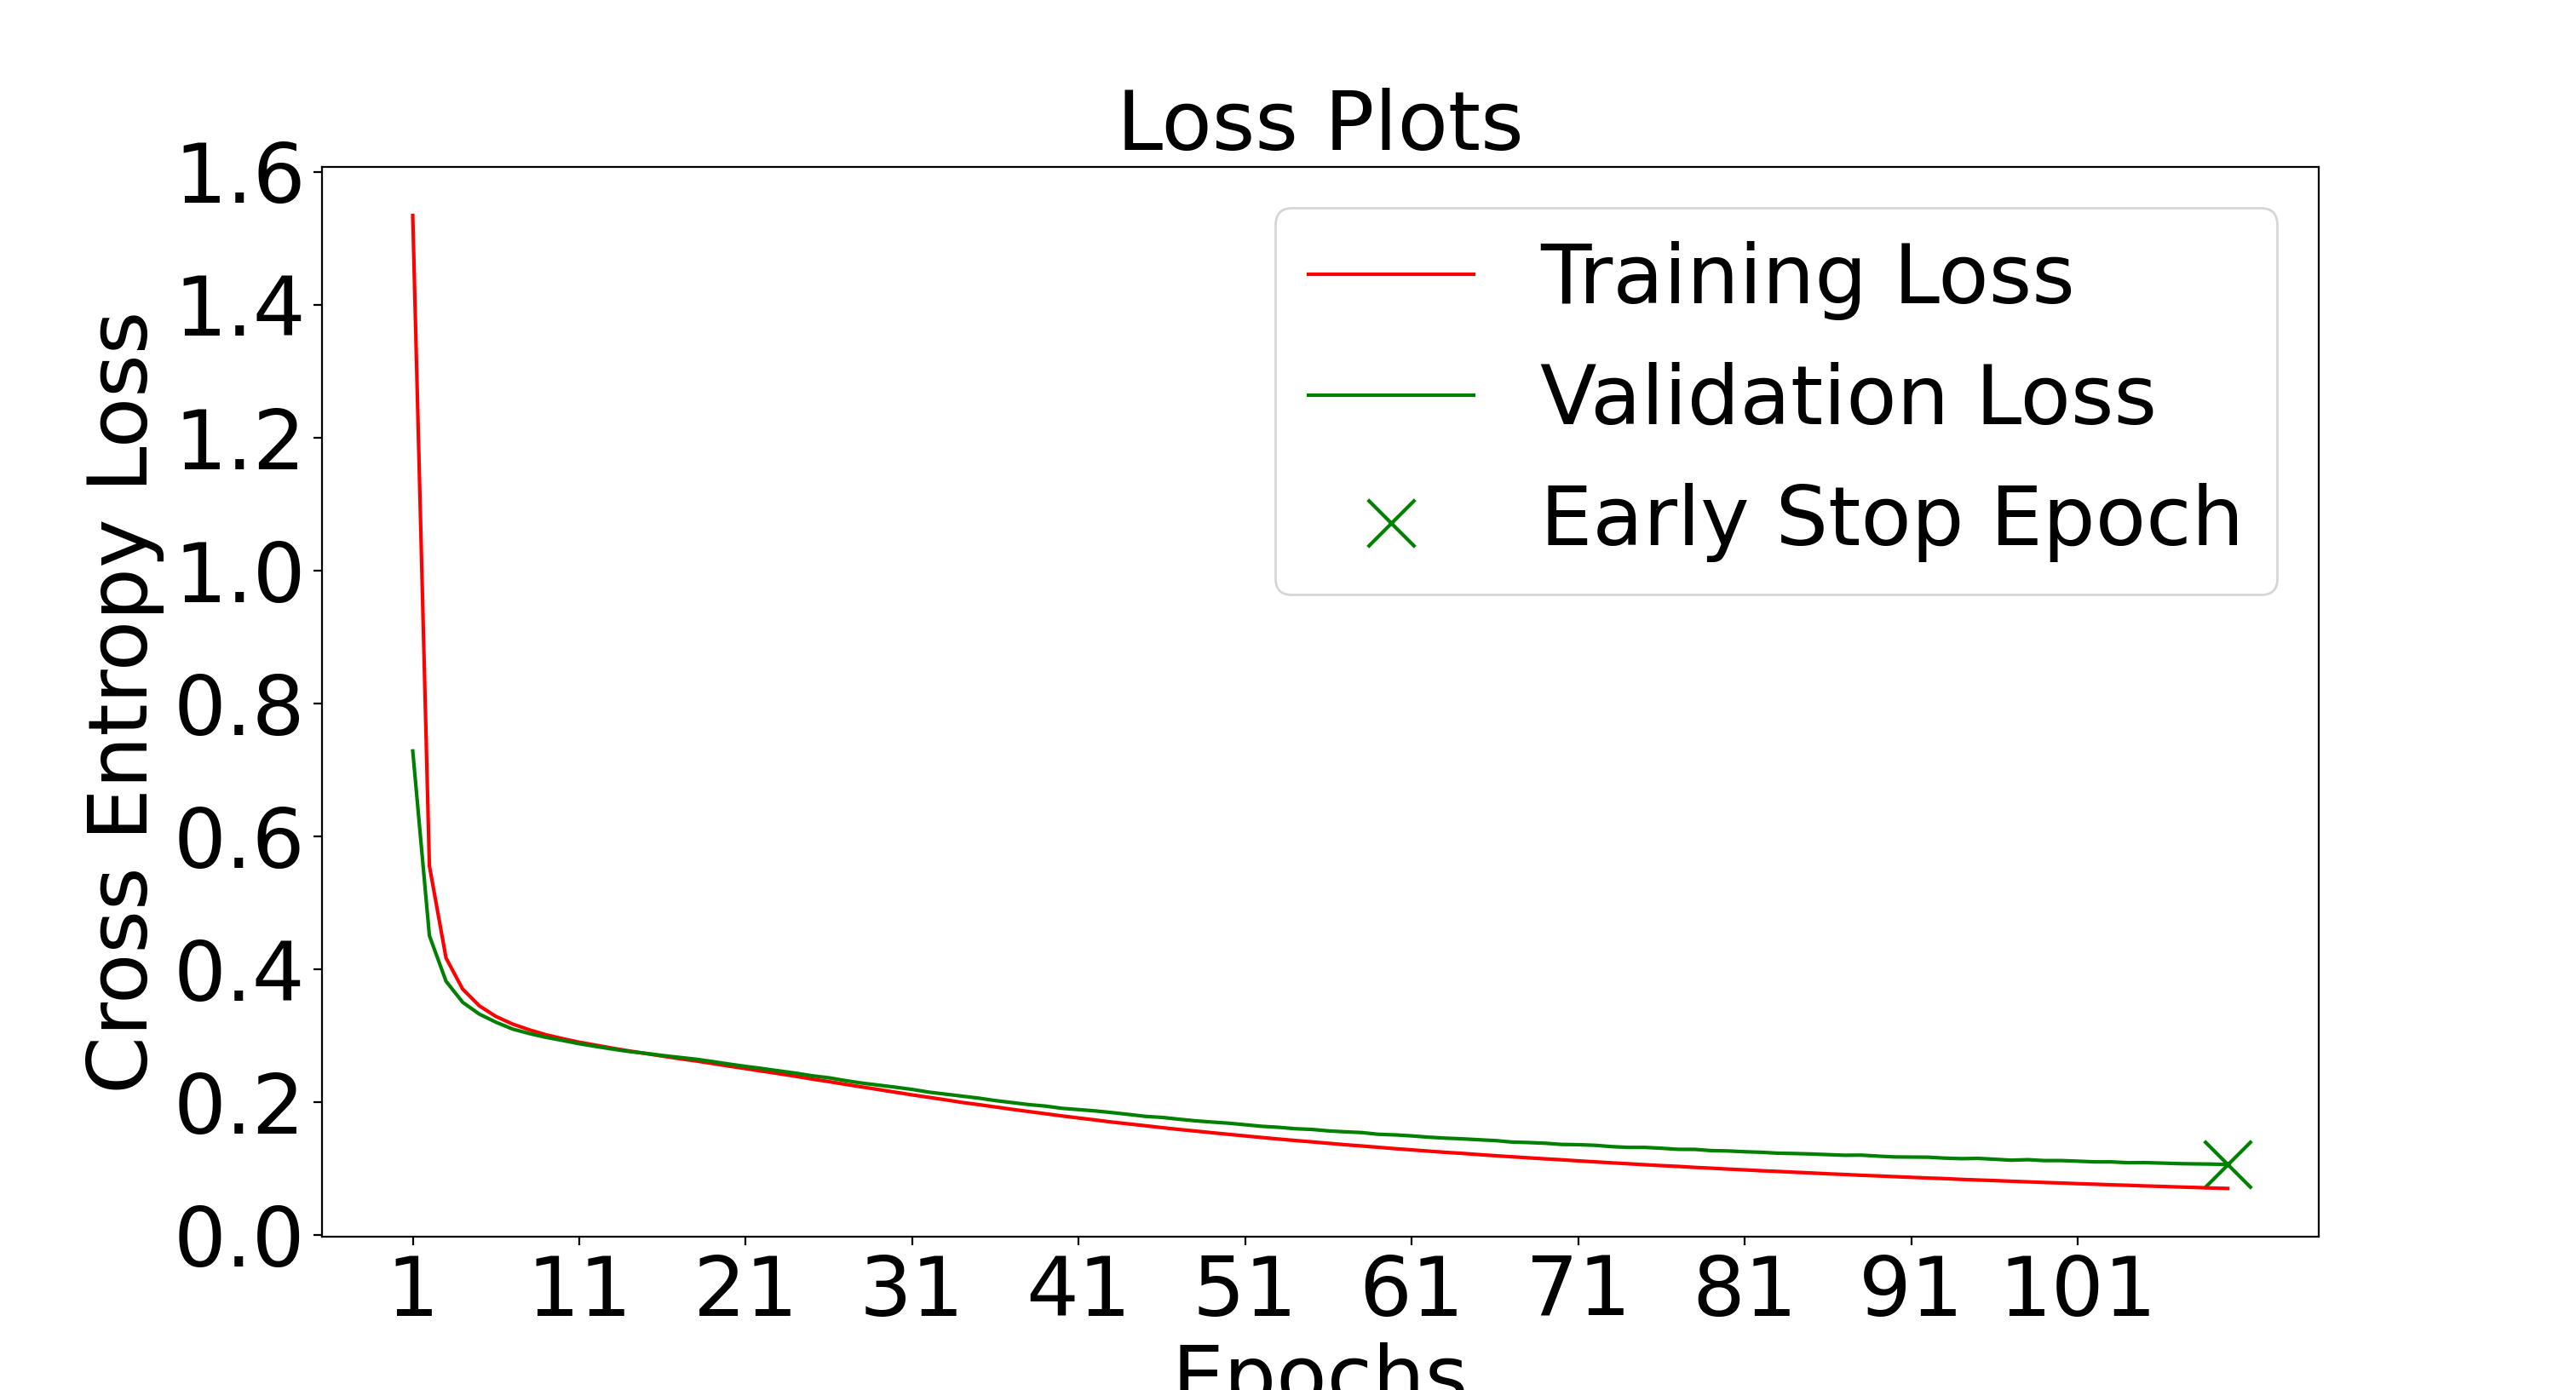
\includegraphics[width=0.8\linewidth]{include/reg-exp-l2-2-loss.png}
  \caption{Train/Validation Loss for L2 Regularization with smaller $\lambda$}
  \label{fig:l2_2_loss}
\end{figure}
\newpage
\subsection{Observations}
\subsubsection{L2 vs L1 regularization}
As can be seen on the both graphs, both the L2 and L1 accuracy graphs are very similar. Both lines on the graph are shaped like a 
negative exponential function with a positive intercept. 
The L1 regularization does have a slightly higher test accuracy than L2, but the difference is not significant since the accuracy difference is only around .004. Similarly, the loss graphs for both regularizations are 
similar since both are shaped as a $e^{-x}$ graph. Also, the
loss of L2 is higher than the loss of L1 by 0.01. One major difference between L1 and L2 regularization is that the L1 regularization required more epochs than
L2 regularization to reach the early stopping condition.

\subsubsection{Smaller $\lambda$ vs Larger $\lambda$}
Both the graphs for accuracy and loss for the smaller lambda vs the larger lambda for 
L2 regularization are very similar. The smaller lambda graph 
has a higher test accuracy than the larger lambda graph by 0.0013.  Also, the loss of 
the smaller lambda is lower than the loss of the larger lambda by 0.001

\section{Activation Experiments}
In this section we did experiments with different activation functions
using mini-batch SGD and the following hyperparameters for all the experiments:
\begin{verbatim}
  learning_rate = 0.01
  batch_size = 128
  epochs = 100
  early_stop = True
  early_stop_epochs = 3
  regularization_type = 'L2'
  L2_penalty = 0.001
  L1_penalty = 0.01
  momentum = True
  momentum_gamma = 0.9
\end{verbatim}
With the layer sizes being $[784, 128, 10]$.

\subsection{Sigmoid Activation}
using the Sigmoid Activation function we got a test accuracy of $0.9336$, and 
a test loss of $0.22483864970441$. The training plots can be seen in
\hyperref[fig:sigmoid_acc]{Figure \ref{fig:sigmoid_acc}} and
\hyperref[fig:sigmoid_loss]{Figure \ref{fig:sigmoid_loss}}.


\begin{figure}[h]
  \centering
  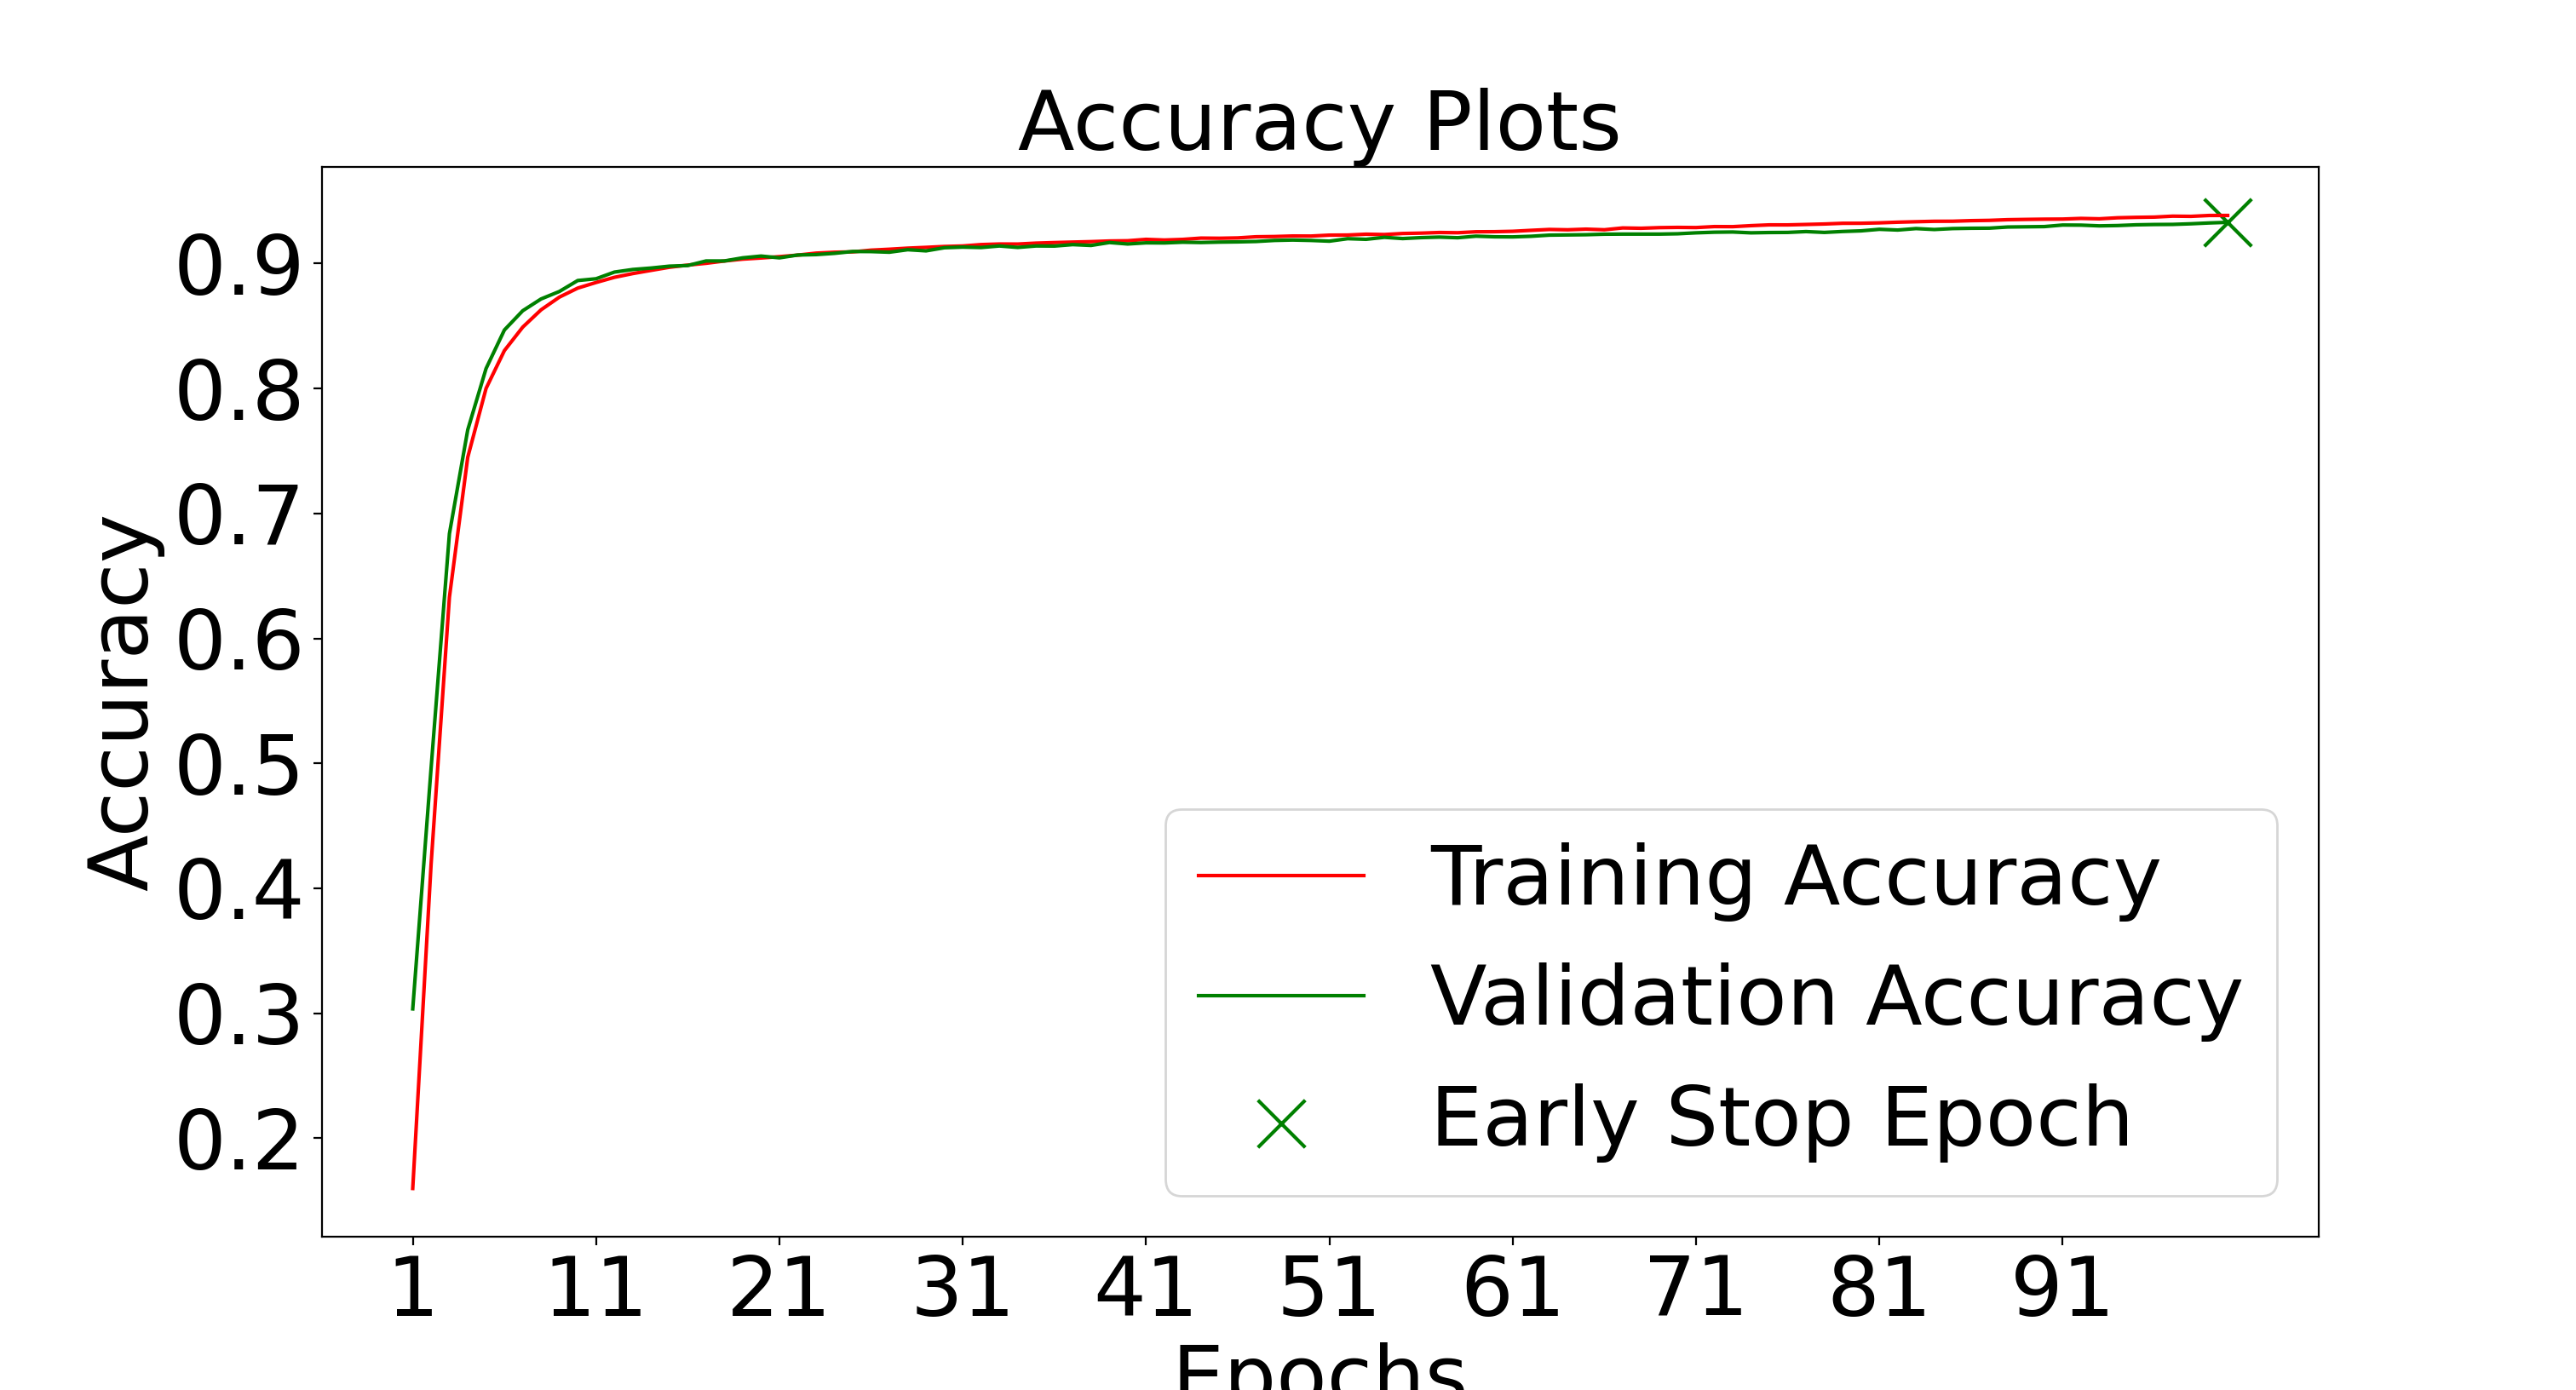
\includegraphics[width=0.8\linewidth]{include/activation-exp-acc-sigmoid.png}
  \caption{Train/Validation Accuracy for Sigmoid}
  \label{fig:sigmoid_acc}
\end{figure}

\begin{figure}[h]
  \centering
  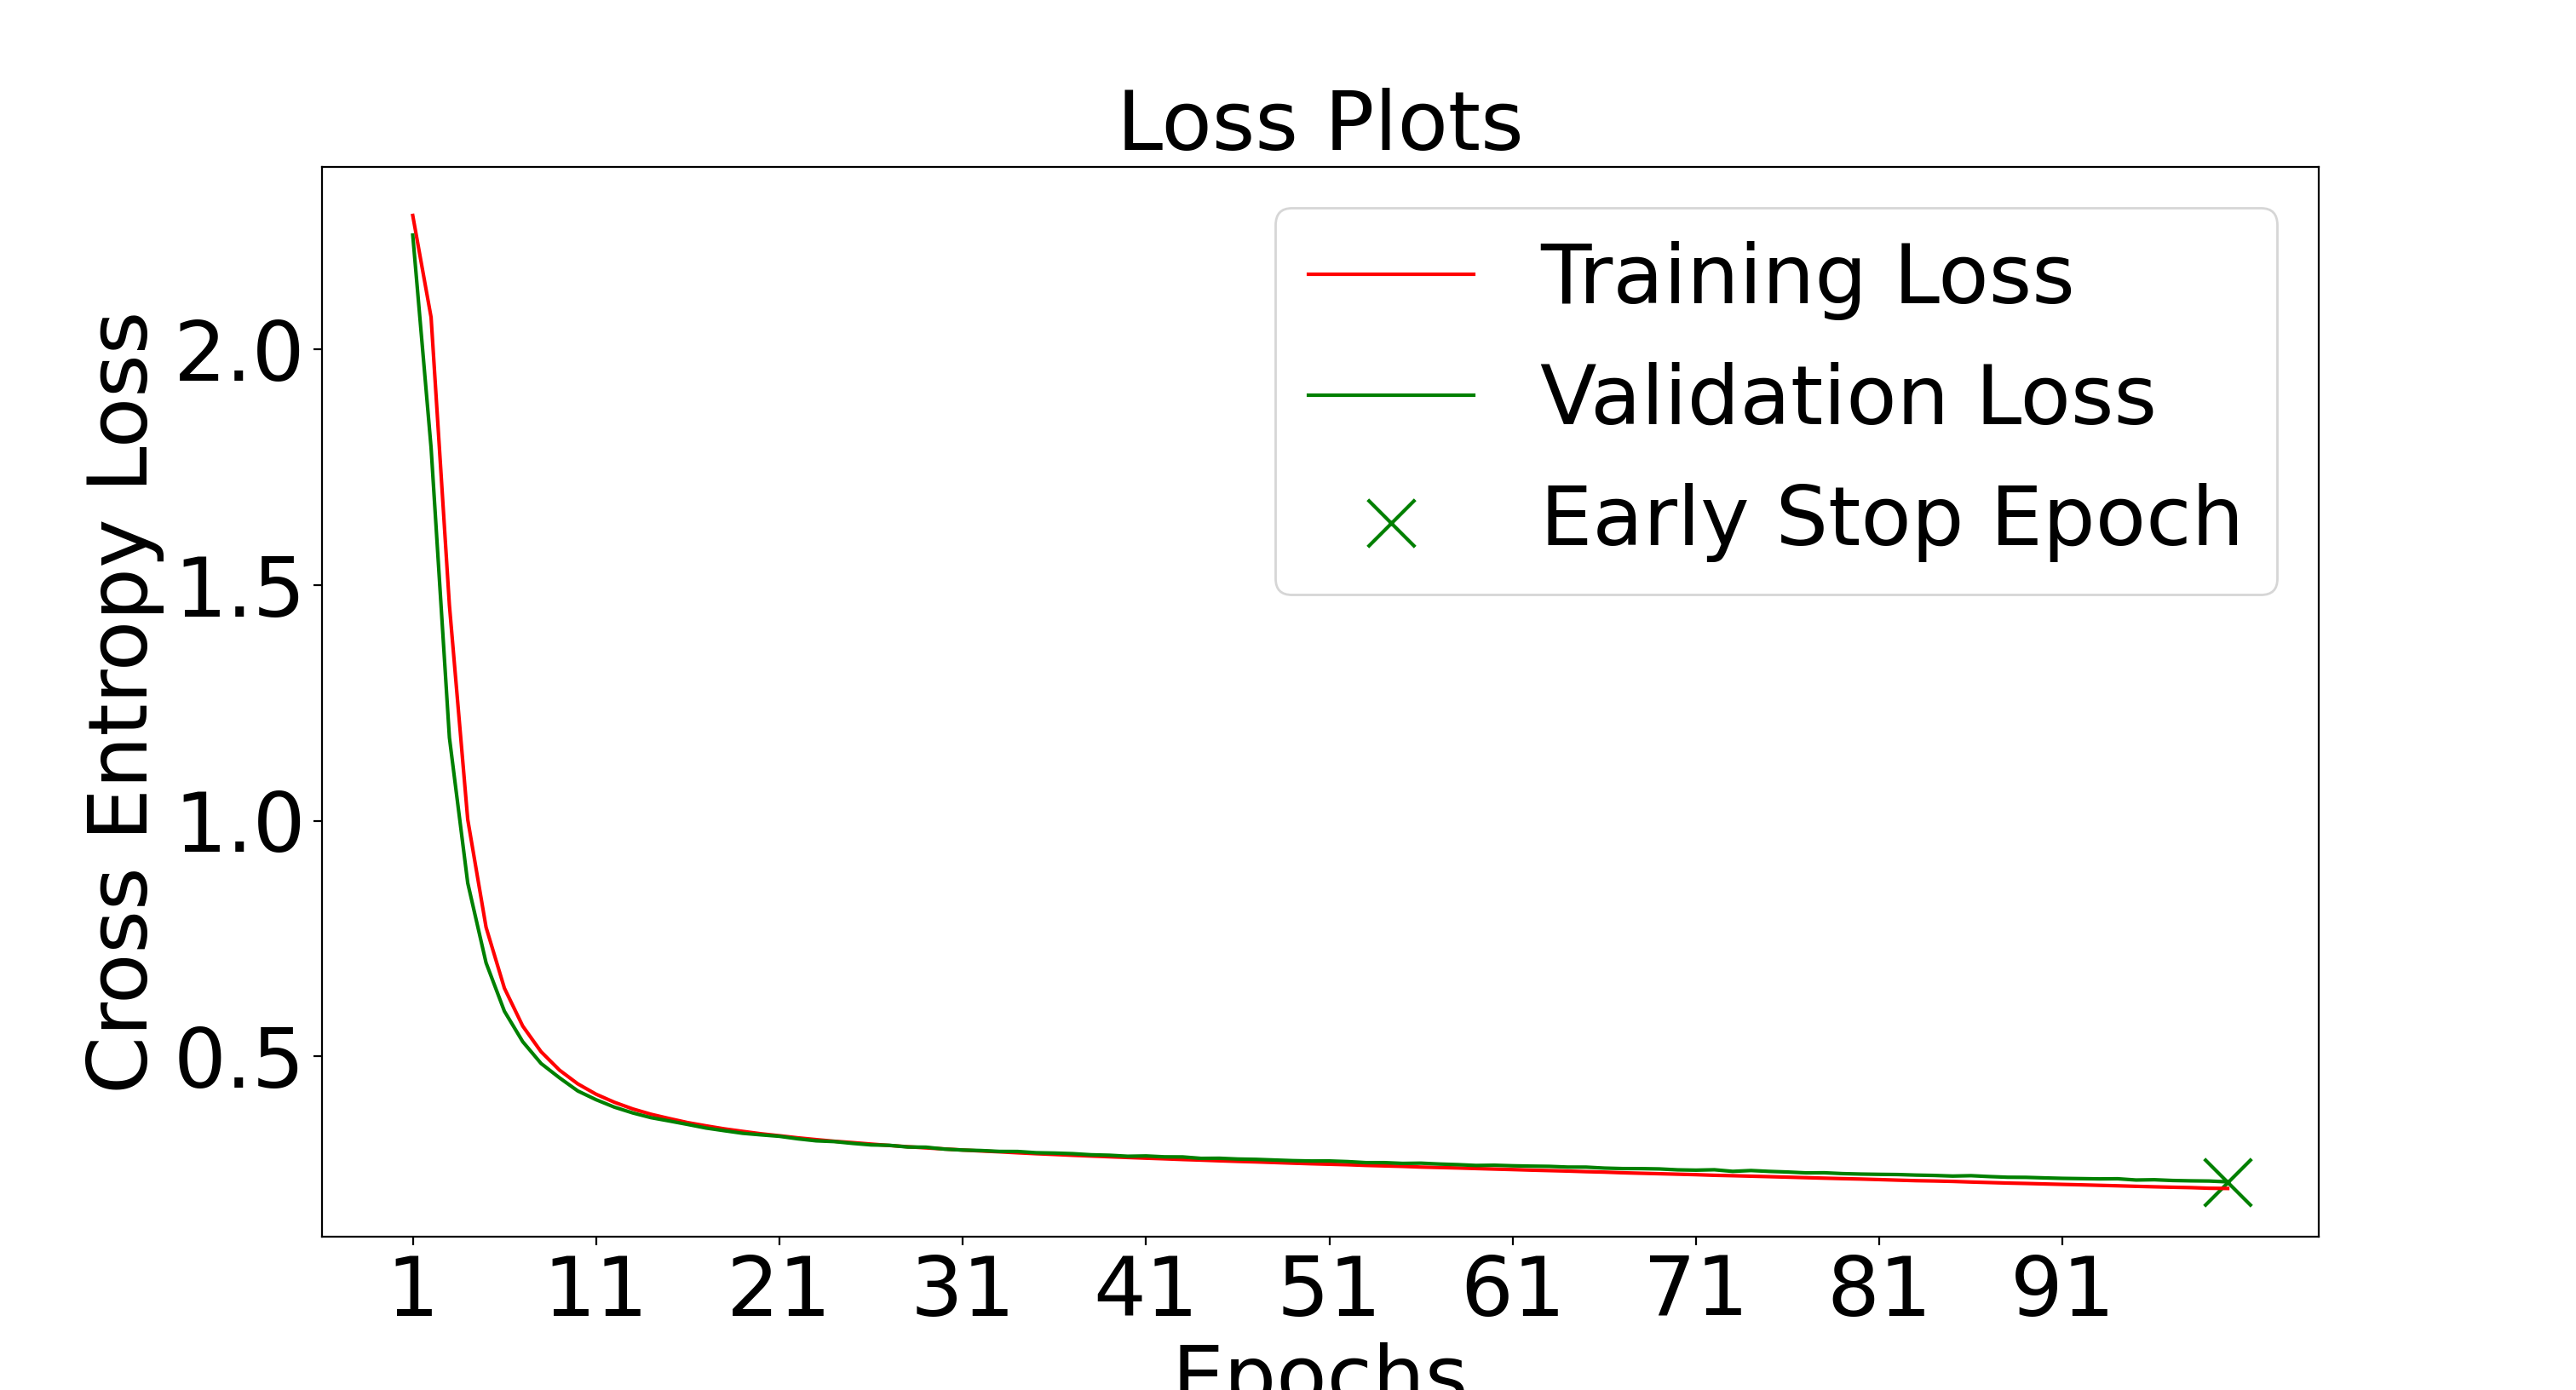
\includegraphics[width=0.8\linewidth]{include/activation-exp-loss-sigmoid.png}
  \caption{Train/Validation Loss for Sigmoid}
  \label{fig:sigmoid_loss}
\end{figure}

\subsection{ReLU Activation}
For the ReLU Activation function we got a test accuracy of $0.9759$ and 
a test loss of $0.080695664408$. The training plots can be seen in
\hyperref[fig:relu_acc]{Figure \ref{fig:relu_acc}} and
\hyperref[fig:relu_loss]{Figure \ref{fig:relu_loss}}.


\begin{figure}[h]
  \centering
  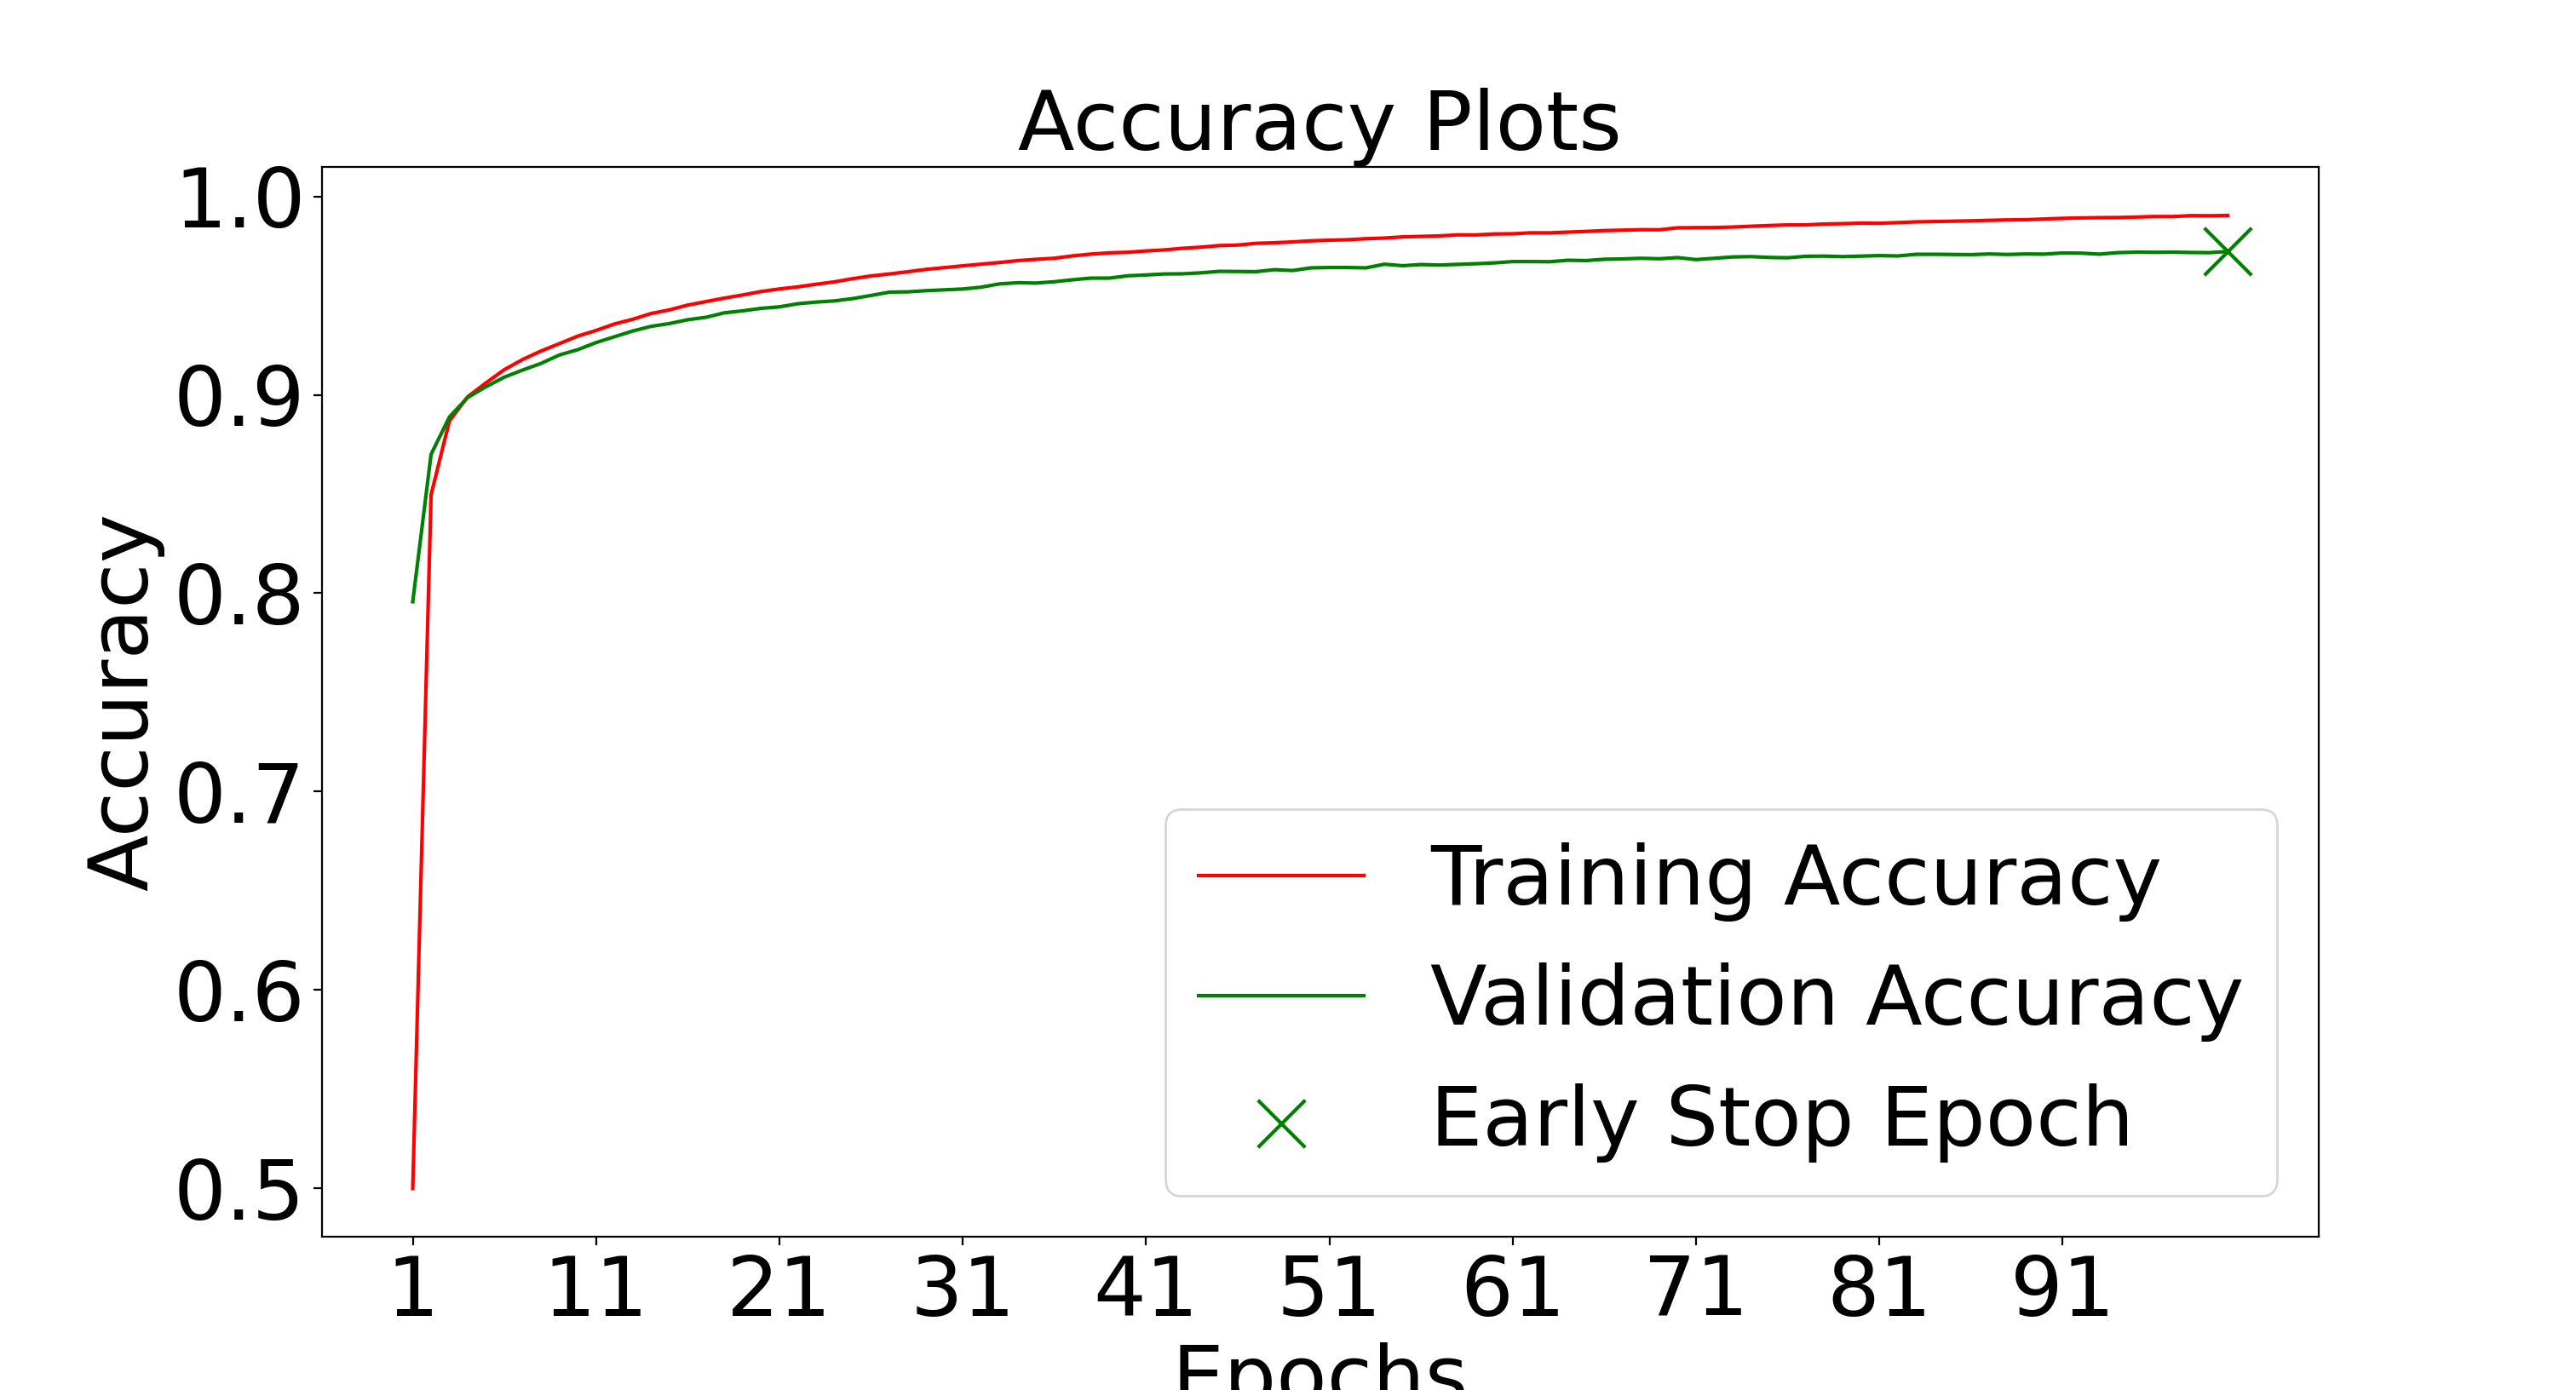
\includegraphics[width=0.8\linewidth]{include/activation-exp-acc-relu.png}
  \caption{Train/Validation Accuracy for ReLU}
  \label{fig:relu_acc}
\end{figure}

\begin{figure}[h]
  \centering
  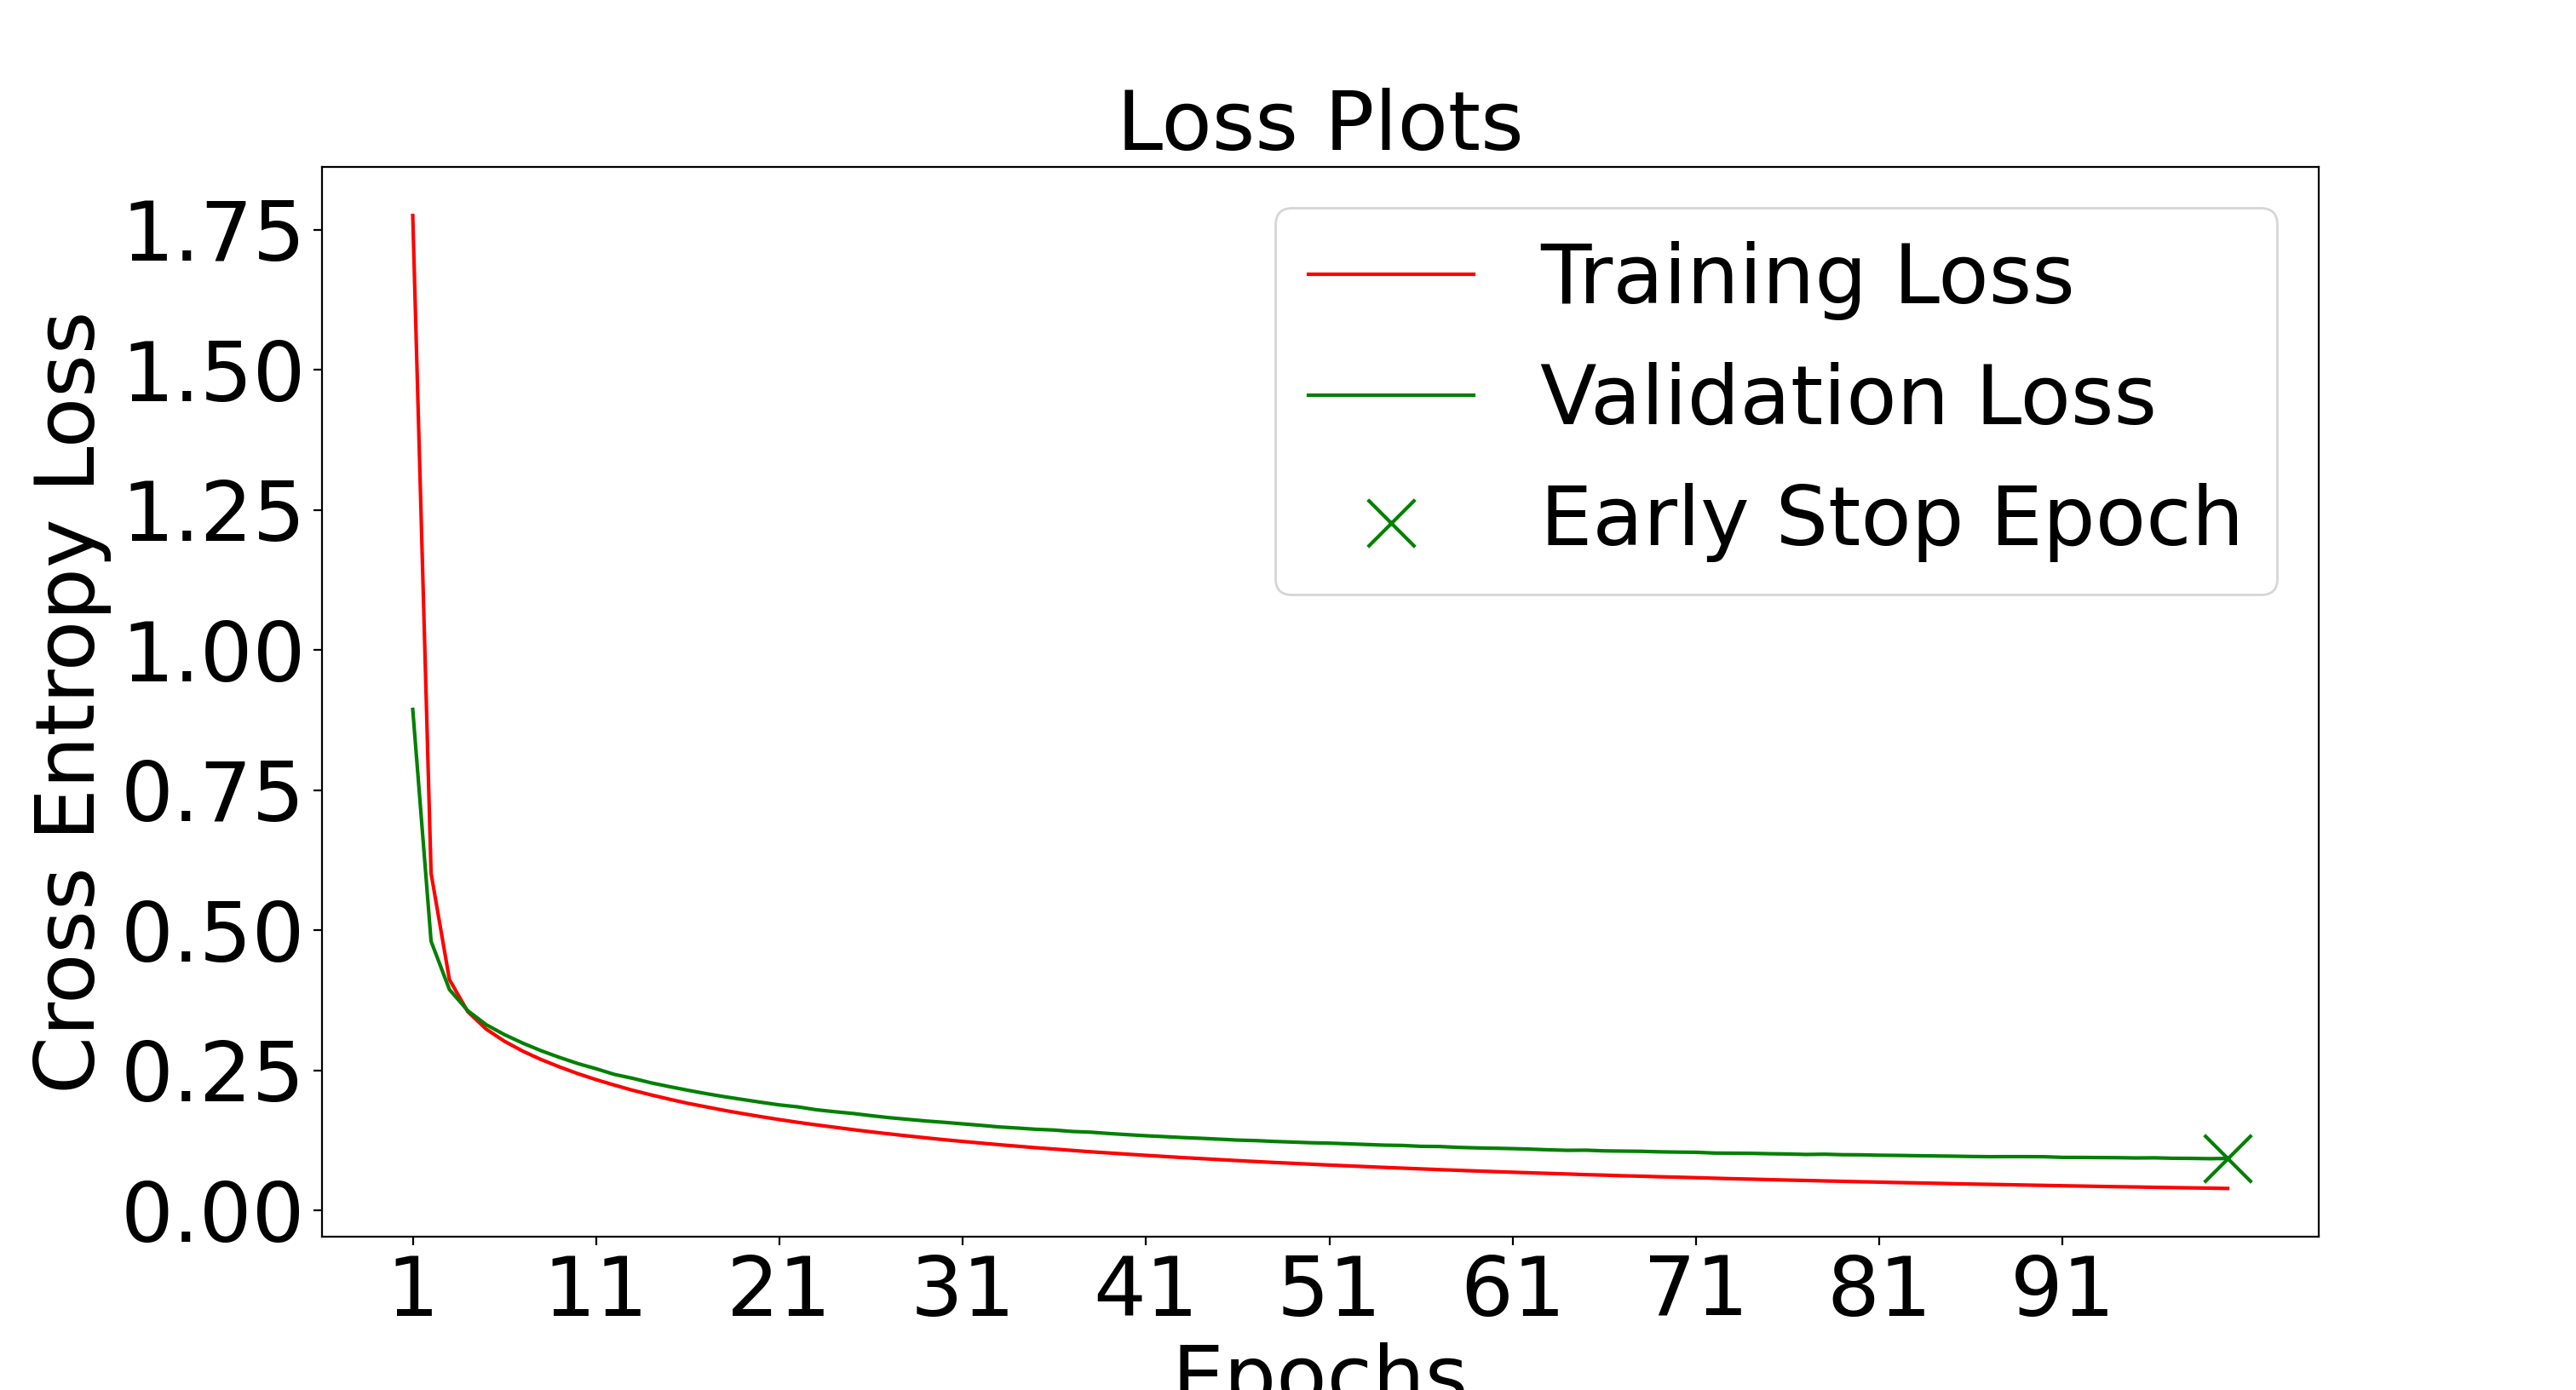
\includegraphics[width=0.8\linewidth]{include/activation-exp-loss-relu.png}
  \caption{Train/Validation Loss for ReLU}
  \label{fig:relu_loss}
\end{figure}

\subsection{Observations}
From what could be observed, the sigmoid activation's test accuracy
 is lower than the ReLU activation's test accuracy, and the sigmoid 
 activation's loss is higher than the ReLU activation's loss. 
 Therefore, it could be implied that in this particular case, the 
 using ReLU as an activation method is more effective than using 
 sigmoid. Another aspect that could be observed is the fact that 
 the both loss graphs are shaped as a negative exponential function. 
 ReLU's losses are less than sigmoid's losses throughout each epoch. 
 In terms of the accuracy graphs, all the lines are shaped as $-e^{-x}$ 
 with a positive intercept. Similar to the loss graphs, ReLU's 
 accuracies are more than sigmoid's accuracies throughout each epoch 
 especially since the ReLU's graphs have a steeper increase.
\section{Best Model}
After some testing the model with the best test accuracy was the model with the following hyperparameters:
\begin{verbatim}
  learning_rate = 0.01
  batch_size = 128
  epochs = 100
  early_stop = True
  early_stop_epochs = 3
  regularization_type = 'L2'
  L2_penalty = 0.001
  L1_penalty = 0.01
  momentum = True
  momentum_gamma = 0.9
\end{verbatim}
With ReLU as the activation function, with a test accuracy of 
$0.9759 \equiv 97.59\%$ and a test loss of $0.080695664408$.



\section{Team Contributions}
Both members contributed equally to the project. We worked together on the
most if not all the code, only have offline work be mostly writing the report
as Jack is fluent with \LaTeX and we did the graphs offline mostly. Another aspect of 
offline work was debugging as we had many bugs and issues with questions 2 and 3
so some offline work from both members was done to debug and fix the issues. 

Otherwise, all the work was done together when we met up in Geisel and worked on the
project together.

%%%%%%%%%%%%%%%%%%%%%%%%%%%%%%%%%%%%%%%%%%%%%%%%%%%%%%%%%%%%
\appendix
\section{Appendix}
\label{sec:appendix}

\subsection{AI Usage}
Here are all the times AI assistance was used in this project (with the prompts)

\subsubsection{Softmax Regression (Overflow Condition) - ChatGPT}
\label{sec:appendix:softmax_overflow-ai}
\textbf{Prompt:} What condition in softmax regression would cause the denominator to become zero and how do we deal with it?

\subsubsection{Clipping the Logits - ChatGPT}
\label{sec:appendix:clipping_logits-ai}
\textbf{Prompt:} 
We are trying to calculate the categorical cross entropy loss for a softmax regression, and we have the Loss function as the following

-np.sum(targets * np.log(logits))

howeverthis is return nans, why and what is causing this

\end{document}